\documentclass[12pt, a4paper]{article}

\usepackage[utf8]{inputenc}
\usepackage[framemethod=TikZ]{mdframed}
\usepackage[hidelinks]{hyperref}
\usepackage{mathtools, amssymb, amsmath, cleveref, fancyhdr, geometry, tcolorbox, graphicx, float, subfigure, arydshln, url, setspace, framed, pifont, physics, ntheorem, utopia}
%%% for coding %%%
\usepackage{listings}
\usepackage[ruled, vlined, linesnumbered]{algorithm2e}

\geometry{a4paper, left=2cm, right=2cm, bottom=2cm, top=2cm}

\pagestyle{fancy}
\fancyhead{}
\fancyhead[L]{\leftmark}
\fancyhead[R]{\rightmark}
\fancyfoot{}
\fancyfoot[C]{\thepage}
%\renewcommand{\headrulewidth}{0pt}
\renewcommand{\footrulewidth}{0pt}

\hypersetup{
	colorlinks = true,
	bookmarks = true,
	bookmarksnumbered = true,
	pdfborder = 001,
	linkcolor = blue
}


\newcounter{index}[subsection]
\setcounter{index}{0}
\newenvironment*{df}[1]{\par\noindent\textbf{Definition \thesubsection.\stepcounter{index}\theindex\ (#1).}}{\par}

\newenvironment*{eg}{\begin{framed}\par\noindent\textbf{Example \thesubsection.\stepcounter{index}\theindex}}{\par\end{framed}}

\newenvironment*{thm}[1]{\begin{tcolorbox}\par\noindent\textbf{Theorem \thesubsection.\stepcounter{index}\theindex\ #1} \par}{\par\end{tcolorbox}}

\newenvironment*{cor}[1]{\par\noindent\textbf{Corollary \thesubsection.\stepcounter{index}\theindex\ #1}}{\par}
\newenvironment*{lem}[1]{\par\noindent\textbf{Lemma \thesubsection.\stepcounter{index}\theindex\ #1}}{\par}
\newenvironment*{ax}[1]{\par\noindent\textbf{Axiom \thesubsection.\stepcounter{index}\theindex\ #1}}{\par}
\newenvironment*{prop}[1]{\par\noindent\textbf{Proposition \thesubsection.\stepcounter{index}\theindex\ #1}}{\par}
\newenvironment*{conj}[1]{\par\noindent\textbf{Conjecture \thesubsection.\stepcounter{index}\theindex\ #1}}{\par}
\newenvironment*{nota}{\par\noindent\textbf{Notation \thesubsection.\stepcounter{index}\theindex.}}{\par}

\newcounter{nprf}[subsection]
\setcounter{nprf}{0}
\newenvironment*{prf}{\par\indent\textbf{\textit{Proof \stepcounter{nprf}\thenprf.}}}{\hfill$\blacksquare$\par}
\newenvironment*{dis}{\par\indent\textbf{\textit{Disproof \stepcounter{nprf}\thenprf.}}}{\hfill$\blacksquare$\par}
\newenvironment*{sol}{\par\indent\textbf{\textit{Solution \stepcounter{nprf}\thenprf.}}\par}{\hfill{$\square$}\par}

\newtheorem*{hint}{Hint.}
\newtheorem*{rmk}{Remark.}
\newtheorem*{ext}{Extension.}

\linespread{1.15}

\title{Emory University\\\textbf{MATH 361 Mathematical Statistics I}\\ Learning Notes}
\author{Jiuru Lyu}
\date{\today}

\def\Z{\mathbb{Z}}
\def\R{\mathbb{R}}
\def\C{\mathbb{C}}
\def\Q{\mathbb{Q}}
\def\N{\mathbb{N}}
\def\d{\mathrm{d}}
\def\epsilon{\varepsilon}
\def\emptyset{\varnothing}
\def\phi{\varphi}
\def\dsst{\displaystyle}
\def\st{\ s.t.\ }
\def\bar{\overline}
\def\E{\vb{E}}
\def\Var{\vb{Var}}
\def\Cov{\vb{Cov}}
\def\P{\vb{P}}
\def\M{\vb{M}}

\newcommand\perm[2][n]{_{#1}P_{#2}}
\newcommand\com[2][n]{_{#1}C_{#2}}

\begin{document}
\maketitle

\tableofcontents

\newpage
\section{Prerequisites}
\begin{df}{Geometric Series}
	A geometric series has the form \[\sum_{n=1}^\infty ar^{n-1}=a+ar+ar^2+\cdots\] If $\qty|r|<1$, then the series converges to $\dfrac{a}{1-r}$. Otherwise, it diverges. 	
\end{df}
\begin{eg}
	Does the series $\dsst\sum_{n=1}^\infty2^{2n}3^{1-n}$ converge or divers?
	\begin{sol}
		Note that \[2^{2n}3^{1-n}=\qty(2^2)^n3^{1-n}=4^n\qty(\dfrac{1}{3})^{n-1}=4\cdot4^{n -1}\qty(\dfrac{1}{3})^{n-1}=4\qty(\dfrac{4}{3})^{n-1}.\] So, \[\sum_{n=1}^\infty2^{2n}3^{1-n}=\sum_{n=1}^\infty4\qty(\dfrac{4}{3})^{n-1}\] is a geometric series, with $a=4$ and $r=\dfrac{4}{3}$.\par Since $\qty|r|=\qty|\dfrac{4}{3}|=\dfrac{4}{3}>1$, the series diverges.
	\end{sol}
\end{eg}
\begin{df}{Taylor Series}
	The Taylor series expanded about $a$ of a differentiable function $f$ is \[f(x)=\sum_{n=0}^\infty\dfrac{f^{(n)}(a)}{n!}(x-a)^n=f(a)+f'(a)(x-a)+\dfrac{f''(a)}{2!}(x-a)^2+\cdots.\]	
\end{df}
\begin{df}{Maclaurin Series}
	The Taylor series expanded about $a=0$.	
\end{df}
\begin{rmk}
	The Maclurin Series of $e^x$ is given by $e^x=\dsst\sum_{n=0}^\infty\dfrac{x^n}{n!}$.	
\end{rmk}
\begin{thm}{Binomial Expansion}
	\[(x+y)^n=\sum_{k=0}^n\binom{n}{k}x^ky^{n-k},\] where $\dsst\binom{n}{k}$ is read as ``$n$ choose $k$'' and can also be written as $nCk$. \[\binom{n}{k}=\dfrac{n!}{k!(n-k)!}=\dfrac{n(n-1)\cdots(n-k+1)}{k!}.\]
\end{thm}
\begin{thm}{Integration by Parts}
	\[\int u\ \d v=uv-\int v\ \d u.\]	
\end{thm}
\begin{eg}
	Evaluate $\dsst\int xe^{-x}\ \d x$.
	\begin{sol}
		Let $u=x,\ \d v=e^{-x}\ \d x$. So, $\d u=\d x$ and $v=\dsst\int e^{-x}\ \d x=-e^{-x}$. Then, \[\int xe^{-x}\ \d x=-xe^{-x}-\int-e^{-x}\ \d x=-xe^{-x}-e^{-x}+C.\]
	\end{sol}
\end{eg}
\begin{df}{Type I Improper Integral}
	If $\dsst\int_a^tf(x)\ \d x$ exists for all $t>0$, then \[\int_a^\infty f(x)\ \d x=\lim_{t\to\infty}\int_a^tf(x)\ \d x.\]
\end{df}
\begin{eg}
	Evaluate $\dsst\int_0^\infty xe^{-x}\ \d x$.
	\begin{sol}
		\[\begin{aligned}\int_0^\infty xe^{-x}\ \d x=\lim_{t\to\infty}\int_0^txe^{-x}\ \d x&=\lim_{t\to\infty}\qty\Big[-xe^{-x}-e^{-x}]_0^t\\&=\lim_{t\to\infty}\qty\Big(-te^{-t}-e^{-t}+1)\\&=-\lim_{t\to\infty}\qty(\dfrac{t}{e^t})-\lim_{t\to\infty}e^{-t}+1\\&=-\lim_{t\to\infty}\qty(\dfrac{1}{e^t})-0+1=-0-0+1=1.\end{aligned}\]
	\end{sol}
\end{eg}
\begin{eg}
	 Double Integrals over Irregular Domains.\\ Consider \[\dsst\iint_D4xy-y^4\ \d A,\] where $D$ is the region bounded between $y=\sqrt{x}$ and $y=x^3$. \par Evaluate this double integral over $D$.
	 \begin{sol}
	 	Firstly, we draw the diagram representing $D$ as follows: 
	 	\begin{center}
	 		\tikzset{every picture/.style={line width=0.75pt}}
	 		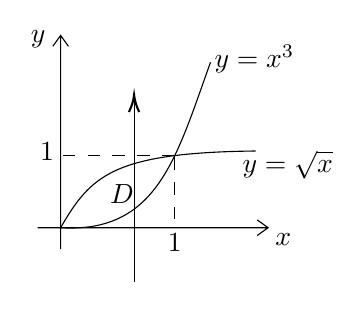
\begin{tikzpicture}[x=0.75pt,y=0.75pt,yscale=-.75,xscale=.75]
	 		\draw  (50,177.55) -- (198.1,177.55)(64.81,54) -- (64.81,191.27) (191.1,172.55) -- (198.1,177.55) -- (191.1,182.55) (59.81,61) -- (64.81,54) -- (69.81,61)  ;
	 		\draw    (64.81,177.55) .. controls (84.1,144.27) and (98.1,129.27) .. (190.1,128.27) ;
	 		\draw    (64.81,177.55) .. controls (127.1,181.27) and (139.1,132.27) .. (161.1,71.27) ;
	 		\draw    (112,212.27) -- (112,94.27) ;
	 		\draw [shift={(112,92.27)}, rotate = 90] [color={rgb, 255:red, 0; green, 0; blue, 0 }  ][line width=0.75]    (10.93,-3.29) .. controls (6.95,-1.4) and (3.31,-0.3) .. (0,0) .. controls (3.31,0.3) and (6.95,1.4) .. (10.93,3.29)   ;
	 		\draw  [dash pattern={on 4.5pt off 4.5pt}]  (138.1,132.27) -- (138.1,177.27) ;
	 		\draw  [dash pattern={on 4.5pt off 4.5pt}]  (138.1,131.27) -- (64.1,131.27) ;
	 		\draw (201,179.4) node [anchor=north west][inner sep=0.75pt]    {$x$};
	 		\draw (44,49.4) node [anchor=north west][inner sep=0.75pt]    {$y$};
	 		\draw (95,148.4) node [anchor=north west][inner sep=0.75pt]    {$D$};
	 		\draw (180,126.4) node [anchor=north west][inner sep=0.75pt]    {$y=\sqrt{x}$};
	 		\draw (162,58.4) node [anchor=north west][inner sep=0.75pt]    {$y=x^{3}$};
	 		\draw (132,179.4) node [anchor=north west][inner sep=0.75pt]    {$1$};
	 		\draw (50,121.4) node [anchor=north west][inner sep=0.75pt]    {$1$};
	 		\end{tikzpicture}
	 	\end{center}
	 	\[\begin{aligned}\iint_D4xy-y^3\ \d A=\int_0^1\int_{x^3}^{\sqrt{x}}4xy-y^3\ \d y\d x&=\int_0^1\qty[2xy^2-\dfrac{1}{4}y^4]_{x^3}^{\sqrt{x}}\ \d x\\&=\int_0^12x\qty(x-x^6)-\dfrac{1}{4}\qty(x^2-x^{12})\ \d x\\&=\int_0^12x^2-2x^7-\dfrac{1}{4}x^2+\dfrac{1}{4}x^{12}\ \d x\\&=\qty[\dfrac{2}{3}x^3-\dfrac{1}{4}x^8-\dfrac{1}{12}x^3+\dfrac{1}{52}x^{13}]_0^1\\&=\dfrac{2}{3}-\dfrac{1}{4}-\dfrac{1}{12}+\dfrac{1}{52}=\dfrac{55}{156}.\end{aligned}\]
	 \end{sol}
\end{eg}

\newpage
\section{Probability}
\subsection{Sample Space and Probability}
\begin{df}{Experiment}
	An \textit{experiment} is a procedure with well-defined outcome.	
\end{df}
\begin{df}{Sample Space/$S$}
	The \textit{sample space}, denoted as $S$ is the set of all possible outcomes of an experiment. 
\end{df}
\begin{df}{Event}
	An \textit{event} is a collection of outcomes.	
\end{df}
\begin{eg}
	Consider flipping two coins. Use $H$ to represent heads and $T$ to represent tails. Then, $S=\qty{HH, HT, TH, TT}$. Event ``one heads''$=\qty{HT, TH}$, and the event ``at least one heads''$=\qty{HT, TH, HH}$.
\end{eg}
\begin{df}{Union/$\cup$}
	$A\cup B$ is the \textit{union} of $A$ and $B$, meaning everything in $A$ and everything in $B$.
\end{df}
\begin{center}
\tikzset{every picture/.style={line width=0.75pt}}
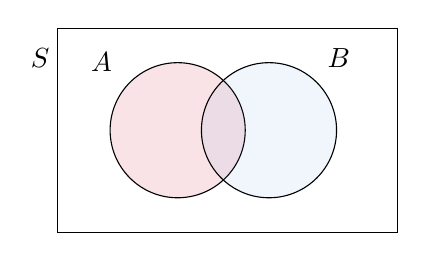
\begin{tikzpicture}[x=0.75pt,y=0.75pt,yscale=-1,xscale=1]
\draw   (111.1,128) -- (275.1,128) -- (275.1,226.27) -- (111.1,226.27) -- cycle ;
\draw  [fill={rgb, 255:red, 208; green, 2; blue, 27 }  ,fill opacity=0.11 ] (136.45,177.14) .. controls (136.45,159.16) and (151.02,144.59) .. (169,144.59) .. controls (186.98,144.59) and (201.55,159.16) .. (201.55,177.14) .. controls (201.55,195.11) and (186.98,209.68) .. (169,209.68) .. controls (151.02,209.68) and (136.45,195.11) .. (136.45,177.14) -- cycle ;
\draw  [fill={rgb, 255:red, 74; green, 144; blue, 226 }  ,fill opacity=0.08 ] (180.45,177.14) .. controls (180.45,159.16) and (195.02,144.59) .. (213,144.59) .. controls (230.98,144.59) and (245.55,159.16) .. (245.55,177.14) .. controls (245.55,195.11) and (230.98,209.68) .. (213,209.68) .. controls (195.02,209.68) and (180.45,195.11) .. (180.45,177.14) -- cycle ;
\draw (126,138.4) node [anchor=north west][inner sep=0.75pt]    {$A$};
\draw (240,136.4) node [anchor=north west][inner sep=0.75pt]    {$B$};
\draw (97,136.4) node [anchor=north west][inner sep=0.75pt]    {$S$};
\end{tikzpicture}	
\end{center}
\begin{df}{Intersection/$\cap$}
	$A\cap B$ is the \textit{intersection} of $A$ and $B$, everything in both $A$ and $B$	
\end{df}
\begin{center}
\tikzset{every picture/.style={line width=0.75pt}}
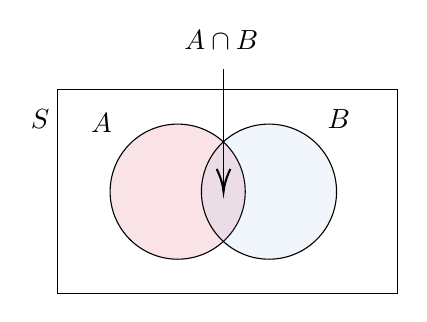
\begin{tikzpicture}[x=0.75pt,y=0.75pt,yscale=-1,xscale=1]
\draw   (111.1,128) -- (275.1,128) -- (275.1,226.27) -- (111.1,226.27) -- cycle ;
\draw  [fill={rgb, 255:red, 208; green, 2; blue, 27 }  ,fill opacity=0.11 ] (136.45,177.14) .. controls (136.45,159.16) and (151.02,144.59) .. (169,144.59) .. controls (186.98,144.59) and (201.55,159.16) .. (201.55,177.14) .. controls (201.55,195.11) and (186.98,209.68) .. (169,209.68) .. controls (151.02,209.68) and (136.45,195.11) .. (136.45,177.14) -- cycle ;
\draw  [fill={rgb, 255:red, 74; green, 144; blue, 226 }  ,fill opacity=0.08 ] (180.45,177.14) .. controls (180.45,159.16) and (195.02,144.59) .. (213,144.59) .. controls (230.98,144.59) and (245.55,159.16) .. (245.55,177.14) .. controls (245.55,195.11) and (230.98,209.68) .. (213,209.68) .. controls (195.02,209.68) and (180.45,195.11) .. (180.45,177.14) -- cycle ;
\draw    (191.1,118.27) -- (191.1,175.14) ;
\draw [shift={(191.1,177.14)}, rotate = 270] [color={rgb, 255:red, 0; green, 0; blue, 0 }  ][line width=0.75]    (10.93,-3.29) .. controls (6.95,-1.4) and (3.31,-0.3) .. (0,0) .. controls (3.31,0.3) and (6.95,1.4) .. (10.93,3.29)   ;
\draw (126,138.4) node [anchor=north west][inner sep=0.75pt]    {$A$};
\draw (240,136.4) node [anchor=north west][inner sep=0.75pt]    {$B$};
\draw (97,136.4) node [anchor=north west][inner sep=0.75pt]    {$S$};
\draw (171,98.4) node [anchor=north west][inner sep=0.75pt]    {$A\cap B$};
\end{tikzpicture}
\end{center}
\begin{df}{Complement/$A^c$}
	$A^c$ denotes the \textit{complement} of $A$, meaning everything in$S$ that is not in $A$.	
\end{df}
\begin{center}
\tikzset{every picture/.style={line width=0.75pt}}
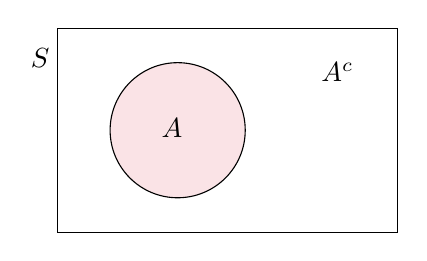
\begin{tikzpicture}[x=0.75pt,y=0.75pt,yscale=-1,xscale=1]
\draw   (111.1,128) -- (275.1,128) -- (275.1,226.27) -- (111.1,226.27) -- cycle ;
\draw  [fill={rgb, 255:red, 208; green, 2; blue, 27 }  ,fill opacity=0.11 ] (136.45,177.14) .. controls (136.45,159.16) and (151.02,144.59) .. (169,144.59) .. controls (186.98,144.59) and (201.55,159.16) .. (201.55,177.14) .. controls (201.55,195.11) and (186.98,209.68) .. (169,209.68) .. controls (151.02,209.68) and (136.45,195.11) .. (136.45,177.14) -- cycle ;
\draw (160,170.4) node [anchor=north west][inner sep=0.75pt]    {$A$};
\draw (97,136.4) node [anchor=north west][inner sep=0.75pt]    {$S$};
\draw (237,143.4) node [anchor=north west][inner sep=0.75pt]    {$A^{c}$};
\end{tikzpicture}	
\end{center}
\begin{cor}{}
	$A\cap A^c=\qty{}=\emptyset$.	
\end{cor}
\begin{df}{Mutually Exclusive}
	Two sets $A$ and $B$ over the same sample space are \textit{mutually exclusive} if they have no outcomes in common. i.e., $A\cap B=\emptyset$.	
\end{df}
\begin{rmk}
	$A$ and $A^c$ are mutually exclusive, but not all sets mutually exclusive are complements of each other.	
\end{rmk}
\begin{df}{Probability Function}
	Let $A$ be an event over a sample space $S$. Then, $\P(A)$ denotes the \textit{probability} of $A$ and $P$ is the \textit{probability function}. The probability function $P$ assigns a number $\P(A)$ for each event $A\subseteq S$.
\end{df}
\begin{ax}{Kolmogorov Axioms}
	\begin{enumerate}
		\item Let $A$ be an event in $S$, then $\P(A)\geq0$.
		\item $\P(S)=1$.
		\item If $A$ and $B$ are mutually exclusive, then $\P(A\cup B)=\P(A)+\P(B)$.
		\item If $A_1,\dots,A_n,\dots$ are mutually exclusive sets, then \[\P\qty(\bigcup_{i=1}^\infty A_i)=\sum_{i=1}^\infty \P(A_i).\]
	\end{enumerate}	
\end{ax}
\begin{prop}{}
	$\P(A^c)=1-\P(A)$.	
\end{prop}
\begin{prf}
	Note that $\P(S)=1$. Since $A^c\cup A=S$, we have $\P(A\cap A^c)=1$. Since $A$ and $A^c$ are mutually exclusive, $\P(A\cup A^c)=\P(A)+\P(A^c)=1$. So, $\P(A^c)=1-\P(A)$.	
\end{prf}
\begin{prop}{}
	$\P(\emptyset)=0$.	
\end{prop}
\begin{prf}
	Note that $\P(S)=1$. Then, $\P(S^c)=1-\P(S)$. By definition, we know $S^c=\emptyset$. So, $\P(\emptyset)=1-\P(S)=1-1=0$.	
\end{prf}
\begin{prop}{}
	$\P(A\cup B)=\P(A)+\P(B)-\P(A\cap B)$	
\end{prop}
\begin{prf}
	Consider the following Venn diagram: 
	\begin{center}
	\tikzset{every picture/.style={line width=0.75pt}}
	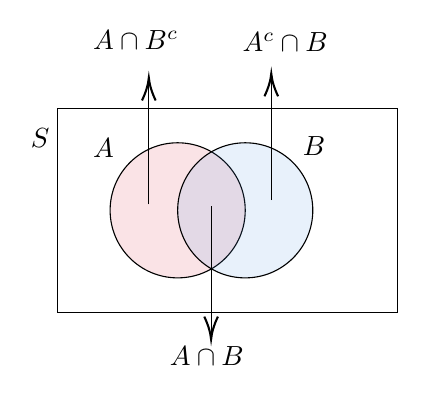
\begin{tikzpicture}[x=0.75pt,y=0.75pt,yscale=-1,xscale=1]
	\draw   (111.1,128) -- (275.1,128) -- (275.1,226.27) -- (111.1,226.27) -- cycle ;
	\draw  [fill={rgb, 255:red, 208; green, 2; blue, 27 }  ,fill opacity=0.11 ] (136.45,177.14) .. controls (136.45,159.16) and (151.02,144.59) .. (169,144.59) .. controls (186.98,144.59) and (201.55,159.16) .. (201.55,177.14) .. controls (201.55,195.11) and (186.98,209.68) .. (169,209.68) .. controls (151.02,209.68) and (136.45,195.11) .. (136.45,177.14) -- cycle ;
	\draw  [fill={rgb, 255:red, 74; green, 144; blue, 226 }  ,fill opacity=0.13 ] (169,177.14) .. controls (169,159.16) and (183.57,144.59) .. (201.55,144.59) .. controls (219.52,144.59) and (234.1,159.16) .. (234.1,177.14) .. controls (234.1,195.11) and (219.52,209.68) .. (201.55,209.68) .. controls (183.57,209.68) and (169,195.11) .. (169,177.14) -- cycle ;
	\draw    (185.1,175.27) -- (185.1,237.27) ;
	\draw [shift={(185.1,239.27)}, rotate = 270] [color={rgb, 255:red, 0; green, 0; blue, 0 }  ][line width=0.75]    (10.93,-3.29) .. controls (6.95,-1.4) and (3.31,-0.3) .. (0,0) .. controls (3.31,0.3) and (6.95,1.4) .. (10.93,3.29)   ;
	\draw    (155.1,174.27) -- (155.1,115.27) ;
	\draw [shift={(155.1,113.27)}, rotate = 90] [color={rgb, 255:red, 0; green, 0; blue, 0 }  ][line width=0.75]    (10.93,-3.29) .. controls (6.95,-1.4) and (3.31,-0.3) .. (0,0) .. controls (3.31,0.3) and (6.95,1.4) .. (10.93,3.29)   ;
	\draw    (214.1,172.27) -- (214.1,113.27) ;
	\draw [shift={(214.1,111.27)}, rotate = 90] [color={rgb, 255:red, 0; green, 0; blue, 0 }  ][line width=0.75]    (10.93,-3.29) .. controls (6.95,-1.4) and (3.31,-0.3) .. (0,0) .. controls (3.31,0.3) and (6.95,1.4) .. (10.93,3.29)   ;
	\draw (127,141.4) node [anchor=north west][inner sep=0.75pt]    {$A$};
	\draw (97,136.4) node [anchor=north west][inner sep=0.75pt]    {$S$};
	\draw (228,140.4) node [anchor=north west][inner sep=0.75pt]    {$B$};
	\draw (127,89.4) node [anchor=north west][inner sep=0.75pt]    {$A\cap B^{c}$};
	\draw (199,90.4) node [anchor=north west][inner sep=0.75pt]    {$A^{c} \cap B$};
	\draw (164,241.4) node [anchor=north west][inner sep=0.75pt]    {$A \cap B$};
	\end{tikzpicture}
	\end{center}
	Note that $\P(A)=\P(A\cap B)+\P(A\cap B^c)$ and $\P(B)=\P(A\cap B)+\P(A^c\cap B)$. So, we have \begin{equation}\label{eq1}\P(A)+\P(B)=\boxed{\P(A\cap B^c)+\P(A^c\cap B)+\P(A\cap B)}+\P(A\cap B).\end{equation} From the Venn diagram, we notice that $\P(A\cap B^c)+\P(A^c\cap B)+\P(A\cap B)$ is exactly $\P(A\cup B)$. So, Eq. (\ref{eq1}) becomes $\P(A)+\P(B)=\P(A\cup B)+\P(A\cap B)$. That is exactly what is required: $\P(A\cup B)=\P(A)+\P(B)-\P(A\cap B)$.
\end{prf}
\begin{df}{Classical Probability}
	In a discrete and finite case, $S$ is finite and all outcomes are equally likely, and the probability function is defined as \[\P(A)=\dfrac{\qty|A|}{\qty|S|},\] where $\qty|A|$ is the cardinality of $A$ and $\qty|S|$ is the cardinality of $S$.	
\end{df}
\begin{eg}
	Despite the definition of classical probability (probability function defined for a discrete and finite case), there are other definitions of probability functions: 
	\begin{enumerate}
		\item Discrete and Countably Infinite: \par Let $S=\N$ be the set of natural numbers. Then, \[\P(k)=\dfrac{1}{2^k}.\] It can also be verified that \[\P(S)=\sum_{k=1}^\infty\dfrac{1}{2^k}=1.\]
		\item Continuous and Uncountably Infinite: \par Let $S=\qty[0,1]$. Suppose $E$ is a subset of $\qty[0,1]$ such that $\dsst\int_E\ \d x$ is defined. Then, \[\P(E)=\int_E\ \d x,\] and it can also be verified that $\P(S)=1$.
	\end{enumerate}	
\end{eg}

\newpage
\subsection{Conditional Probability and Independence}
\begin{df}{Conditional Probability}
	We read $\P(A|B)$ as the probability of $A$ given $B$. Knowing $B$ occurs, we create a new sample space, in which the probability of $A$ occurs changes: \[\P(A|B)=\dfrac{\qty|A\cap B|}{\qty|B|}=\dfrac{\qty|A\cap B|}{\qty|B|}\cdot\dfrac{1/\qty|S|}{1/\qty|S|}=\dfrac{\qty|A\cap B|/\qty|S|}{\qty|B|/\qty|S|}=\dfrac{\P(A\cap B)}{\P(B)}.\]	
\end{df}
\begin{cor}{}
	$\P(A\cap B)=\P(A|B)\P(B)$
\end{cor}
\begin{eg}
	Find the probability of dealing $A$ first, $2$ second, and $3$ third.
	\begin{sol}
		\[\begin{aligned}\P(\text{dealing }A,2,3)&=\P(A\text{ first})\P(2\text{ second}|A\text{ first})\P(3\text{ third}|A\text{ first}\cap2\text{ second})\\&=\dfrac{4}{52}\cdot\dfrac{4}{51}\cdot\dfrac{4}{50}\end{aligned}\]
	\end{sol}
\end{eg}
\begin{cor}{}
	$\P(A_1\cap A_2\cap A_3)=\P(A_1)\P(A_2|A_1)\P(A_3|A_2\cap A_1).$	
\end{cor}
\begin{thm}{The Law of Total Probability}
	Suppose the sample space $S=A_1\cup A_2\cup\cdots\cup A_n$, with $A_i\cap A_j=\emptyset\quad\forall i\neq j$	. Then, \[\P(B)=\P(B\cap A_1)+\P(B\cap A_2)+\cdots+\P(B\cap A_n).\]
\end{thm}
\begin{rmk}
	This theorem gives us a nice way to partition the sample space. 	
\end{rmk}
\begin{eg}
	\begin{center}
	\tikzset{every picture/.style={line width=0.75pt}}
	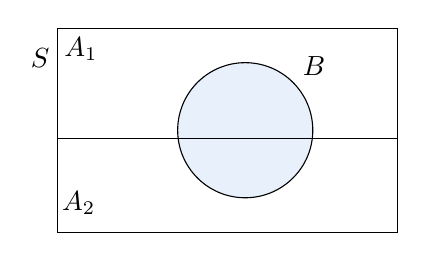
\begin{tikzpicture}[x=0.75pt,y=0.75pt,yscale=-1,xscale=1]
	\draw   (111.1,128) -- (275.1,128) -- (275.1,226.27) -- (111.1,226.27) -- cycle ;
	\draw  [fill={rgb, 255:red, 74; green, 144; blue, 226 }  ,fill opacity=0.13 ] (169,177.14) .. controls (169,159.16) and (183.57,144.59) .. (201.55,144.59) .. controls (219.52,144.59) and (234.1,159.16) .. (234.1,177.14) .. controls (234.1,195.11) and (219.52,209.68) .. (201.55,209.68) .. controls (183.57,209.68) and (169,195.11) .. (169,177.14) -- cycle ;
	\draw    (111,181) -- (275,181) ;
	\draw (113.1,131.4) node [anchor=north west][inner sep=0.75pt]    {$A_{1}$};
	\draw (97,136.4) node [anchor=north west][inner sep=0.75pt]    {$S$};
	\draw (228,140.4) node [anchor=north west][inner sep=0.75pt]    {$B$};
	\draw (112.1,205.4) node [anchor=north west][inner sep=0.75pt]    {$A_{2}$};
	\end{tikzpicture}
	\end{center}
	As represented in the diagram above, $\P(B)=\P(B\cap A_1)+\P(B\cap A_2)$. 
\end{eg}
\begin{thm}{Bayes Theorem}
	\[\P(B|A)=\dfrac{\P(A\cap B)}{\P(A)}=\dfrac{\P(A|B)\P(B)}{\P(A|B)\P(B)+\P(A|B^c)\P(B^c)}.\]	
\end{thm}
\begin{eg}{}
	Coronary Artery Disease (CAD)
	\par The probability of someone having CAD is 60\%. In a study of 101 patients, 37 of them are known to NOT have CAD and 64 are known to have CAD. Of the 37 patients without CAD, 34 had negative tests while 3 had positive tests. Of the 64 with CAD, 54 had positive tests and 10 had negative tests. Find the probability of a patient has CAD given positive test.
	\begin{sol}
		Let $T+$ be positive test, $T-$ be negative test, $D+$ be presence of CAD, and $D-$ be absence of CAD. Then, from the problem, we have \[\P(D+)=0.6;\quad \P(D-)=1-\P(D+)=0.4\] and \[\P(T+|D+)=\dfrac{54}{64}\approx0.84;\quad \P(T-|D-)=\dfrac{34}{37}\approx0.92;\quad \P(T+|D-)=\dfrac{3}{37}\approx0.08.\] Then, by Bayes Theorem, \[\begin{aligned}\P(D+|T+)&=\dfrac{\P(T+|D+)\P(D+)}{\P(T+|D+)\P(D+)+\P(T+|D-)\P(D-)}\\&=\dfrac{0.84\times0.6}{0.84\times0.6+0.08\times0.4}\approx\boxed{0.94}.\end{aligned}\]
	\end{sol}
\end{eg}
\begin{df}{Independence}
	Events $A$ and $B$ are \textit{independent} if $\P(A|B)=\P(A)$, meaning the occurrence of $B$ does note affect the occurrence of $A$.
\end{df}
\begin{cor}{}
	If $A$ and $B$ are independent, then $\P(A\cap B)=\P(A|B)\P(B)=\P(A)\P(B).$
\end{cor}
\begin{eg}{Draw a card from 52 card deck}
	\par Let $A$: The card is an Ace and $H$: The card is a hearts. Then, \[\P(A\cap H)=\P(\text{The card is an Ace of hearts})=\dfrac{1}{52}=\dfrac{1}{4}\cdot\dfrac{1}{13}=\P(H)\P(A).\] So, ranks and suits are independent. 
\end{eg}
\begin{eg}{}
	Mutually Exclusive v.s. Independence
	\par A coin is flipped twice: $S=\qty{HH, TH, HT, TT}$. Let $A=\text{The first flip is }H=\qty{HH,HT}$ and $B=\text{The second flip is }T=\qty{HT,TT}$.
	\begin{itemize}
		\item $A$ and $B$ are independent: $A\cap B=\qty{HT}$. So, $\P(A\cap B)=\dfrac{1}{4}$. Since $\P(A\cap B)\dfrac{1}{4}=\dfrac{1}{2}\cdot\dfrac{1}{2}=\P(A)\P(B)$, we know $A$ and $B$ are independent. 
		\item $A$ and $B$ are not mutually exclusive because $\P(A\cap B)=\dfrac{1}{4}\neq0$.
	\end{itemize}
\end{eg}
\begin{df}{Repeated Trials}
	A sequence of events $A_1,\dots,A_n$ is called independent if for any combination \[\P(A_{i1}\cap A_{i2}\cap\cdots\cap A_{ik})=\P(A_{i1})\P(A_{i2})\cdots \P(A_{ik}).\] In this case, each individual event is  called a \textit{trial}.
\end{df}
\begin{eg}{}
	Roll a fair die repeatedly. What is the probability that the first $6$ appears on the roll $k$? If I win when $6$ is rolled, what is the probability that I win? 
	\begin{sol}
		Let $A_j=\text{the first }6\text{ is rolled on roll }j$.
		\begin{center}\begin{tabular}{ll}
		$j=1$&$\P(A_1)=\dfrac{1}{6}$\\\\
		$j=2$&$\P(A_2)=\qty(\dfrac{5}{6})\qty(\dfrac{1}{6})$\\\\
		$j=3$&$\P(A_3)=\qty(\dfrac{5}{6})\qty(\dfrac{5}{6})\qty(\dfrac{1}{6})=\qty(\dfrac{5}{6})^2\qty(\dfrac{1}{6})$\\\\
		$j=4$&$\P(A_4)=\qty(\dfrac{5}{6})^3\qty(\dfrac{1}{6})$\\
		$\vdots$&\\
		$j=k$&$\P(A_k)=\qty(\dfrac{5}{6})^{k-1}\qty(\dfrac{1}{6})$
		\end{tabular}\end{center}
		So, \[\begin{aligned}\P(\text{I win})&=\P(A_1)+\P(A_2)+\cdots+\P(A_k)+\cdots\\&=\dfrac{1}{6}+\qty(\dfrac{5}{6})\qty(\dfrac{1}{6})+\cdots+\qty(\dfrac{5}{6})^{k-1}\qty(\dfrac{1}{6})+\cdots\\&=\qty(\dfrac{1}{6})\qty(1+\qty(\dfrac{5}{6})+\cdots+\qty(\dfrac{5}{6})^{k-1}+\cdots)\\&=\qty(\dfrac{1}{6})\sum_{i=0}^\infty\qty(\dfrac{5}{6})^i=\dfrac{1}{6}\cdot\dfrac{1}{1-\dfrac{5}{6}}=\dfrac{1}{6}\cdot6=\boxed{1}.\end{aligned}\]
	\end{sol}
\end{eg}
\begin{eg}{}
	Three people $A,B$ and $C$ take turn to flip a coin. Whoever gets a heads wins. Find the probability of each individual winning. 
	\begin{sol}
		First consider the case when Player $A$ wins. Let $A_j=\text{Player }A\text{ wins on the }j\text{-th turn}$. 
		\begin{center}\begin{tabular}{ll}
		$j=1$&$\P(A_1)=\dfrac{1}{2}$\\\\
		$j=2$&$\P(A_2)=\qty(\dfrac{1}{2}\cdot\dfrac{1}{2}\cdot\dfrac{1}{2})\qty(\dfrac{1}{2})$\\\\
		$j=3$&$\P(A_3)=\qty(\dfrac{1}{2}\cdot\dfrac{1}{2}\cdot\dfrac{1}{2})\qty(\dfrac{1}{2}\cdot\dfrac{1}{2}\cdot\dfrac{1}{2})\qty(\dfrac{1}{2})=\qty(\dfrac{1}{2}\cdot\dfrac{1}{2}\cdot\dfrac{1}{2})^2\qty(\dfrac{1}{6})$\\\\
		$j=4$&$\P(A_4)=\qty(\dfrac{1}{2}\cdot\dfrac{1}{2}\cdot\dfrac{1}{2})^3\qty(\dfrac{1}{2})$\\
		$\vdots$&\\
		$j=k$&$\P(A_k)=\qty(\dfrac{1}{2}\cdot\dfrac{1}{2}\cdot\dfrac{1}{2})^{k-1}\qty(\dfrac{1}{2})=\qty(\dfrac{1}{8})^{k-1}\qty(\dfrac{1}{2})$
		\end{tabular}\end{center}	
		So, \[\begin{aligned}\P(A\text{ wins})=\sum_{j=1}^\infty \P(A_j)&=\dfrac{1}{2}+\qty(\dfrac{1}{8})\qty(\dfrac{1}{2})+\cdots+\qty(\dfrac{1}{8})^{k-1}\qty(\dfrac{1}{2})+\cdots\\&=\dfrac{1}{2}\sum_{i=0}^\infty\qty(\dfrac{1}{8})^i\\&=\dfrac{1}{2}\cdot\dfrac{1}{1-\dfrac{1}{8}}=\dfrac{1}{2}\cdot\dfrac{8}{7}=\boxed{\dfrac{4}{7}}.\end{aligned}\]
		Similarly, we can get the probability of player $B$ wins to be $\P(B\text{ wins})=\dfrac{2}{7}$. Finally, we can compute the probability of player $C$ wins by \[\P(C\text{ wins})=1-\P(A\text{ wins})-\P(B\text{ wins})=1-\dfrac{4}{7}-\dfrac{2}{7}=\dfrac{1}{7}.\]
	\end{sol}
\end{eg}

\subsection{Combinatorics}
\begin{thm}{Multiplication Rule}
	If operation $A$ can be performed in $n$ ways and operation $B$ in $m$ ways, then the sequence (operation $A$, operation $B$) can be performed in $n\times m$ ways.	
\end{thm}
\begin{cor}{Ordered Sequence}
	Consider a set $A$ and $\qty|A|=n$. Then, an \textit{ordered sequence} of $A$, $(x_1,x_2,\dots,x_k)\st x_i\in A$, is picked with replacement of elements. Then, \[\qty|(x_1,x_2,\dots,x_k)|=n^k.\]	
\end{cor}
\begin{rmk}
	In this situation, repetition is allowed. 	
\end{rmk}
\begin{df}{Permutation}
	\textit{Permutation} is an ordered sequence without replacement of elements. That is, $(x_1,x_2,\dots,x_k)\st x_i\in A$ and $x_i\neq x_j\forall i\neq j$. Then, \[\qty|(x_1,x_2,\dots,x_k)|=n(n-1)\cdots(n-k+1).\] It is also written as $\perm[n]{k}=\dfrac{n!}{(n-k)!}$.
\end{df}
\begin{df}{Combination}
	\textit{Combination} is an unordered permutation (no order, no replacement of elements). So, we have \begin{align*}\text{permutation}&=\text{combination}\times\text{orderings}\\\perm[n]{k}&=\com[n]{k}\times k!\\\com{k}&=\dfrac{\perm{k}}{k!}=\dfrac{n!}{(n-k)!k!}=\binom{n}{k}\end{align*}
\end{df}
\begin{rmk}
	People are always distinct. Letter or coins are not usually distinct. 	
\end{rmk}
\begin{eg}
	How many ways can we scramble the letters in STATISTICS? 
	\begin{sol}
		If the letter are distinct, then $10!$ ways to scramble the word. However, they are not distinct: 
		\begin{center}\begin{tabular}{c|c}
			Non-distinct Letters&Ways to Scramble\\\hline
			$S - 3$&$3!$\\
			$T - 3$&$3!$\\
			$I - 2$&$2!$
		\end{tabular}\end{center}
		So, ways to scramble the word $N$ satisfies \begin{align*}10!&=N\cdot3!\cdot3!\cdot2!\\N&=\dfrac{10!}{3!\cdot3!\cdot2!}\quad\text{Multinomial Coefficient}\end{align*}
	\end{sol}
\end{eg}
\begin{df}{Multinomial Coefficient}
	The \textit{multinomial coefficient} is the number of ways that $n$ objects with $n_j$ of type $j$, where $j=1,\dots,r$, can be distinctly ordered. So, \[\sum_{j=1}^rn_j=n\] and \[\text{Multinomial Coefficient}=\dfrac{n!}{n_1!\cdot n_2!\cdot\cdots\cdot n_r!}\]
\end{df}
\begin{rmk}
	Tips for Counting:
	\begin{enumerate}
		\item Draw a picture of the structure
		\item Construct a smaller problem when there are large numbers or variables.
		\item If the structure of the problem falls into different categories, then add instead of multiple. 
	\end{enumerate}	
\end{rmk}

\subsection{Combinatorial Probabilities}
\begin{rmk}
	Probability Tips
	\begin{enumerate}
		\item Avoid multiplying probabilities. Always set up quotient.
		\item Keep track of order. If we have order in the sample space, we will need order in the event.
		\item Know some basic sample spaces:
		\begin{itemize}
			\item Rolling $n$ fair die: $\qty|S|=6^n$ (ordered).
			\item Flipping $n$ coins: $\qty|S|=2^n$
			\item Dealing a hand of $n$ cards: $\dsst\binom{52}{n}$
		\end{itemize}
	\end{enumerate}	
\end{rmk}
\begin{eg}{}
	Roll $5$ Fair Die. What is the size of the sample space? What is the probability that the first three have one face and the last two another? What is the probability that two faces show up exactly twice? 
	\begin{sol}
		\par Size of the sample space: $\qty|S|=6^5$.
		\par Let $A=$ the probability that the first three have one face and the last two another. $\qty|A|=(6\times1\times1)\times(5\times1)=30$. So, $\P(A)=\dfrac{30}{6^5}=\dfrac{5}{6^4}$.
		\par Let $B=$ the probability that two faces show up exactly twice. Note that we use $\dsst\binom{6}{2}$ to give the faces of the pairs. $\dsst\binom{4}{1}$ to the last one. $\dfrac{5!}{2!\cdot2!\cdot1!}$ ways to order the faces. So, $\qty|B|=\dsst\binom{6}{2}\binom{4}{1}\dfrac{5!}{2!\cdot2!\cdot1!}$. Then, $\P(B)=\dfrac{\binom{6}{2}\binom{4}{1}\frac{5!}{2!\cdot2!\cdot1!}}{6^5}$.
	\end{sol}
\end{eg}

\newpage
\section{Random Variables}
\subsection{Discrete RV: Binomial \& Hypergeometric}
\begin{df}{Random Variable}
	A \textit{random variable} is a number determined by the outcome of an experiment, $X:S\to\R$. Usually, we are not particularly interested in $S$ but in the distribution of the outcomes for $X$. We want to describe the probability associated with different values of $X$.
\end{df}
\begin{eg}
	Flip three coins. Count the number of heads ($H$): \[S=\qty{HHH, HHT, HTH, TTH TTH THT, HTT, TTT}\] \[\widetilde{S}=\qty{3H, 2H, 1H, 0H}.\] Note in $\widetilde{S}$, not every outcome is equally likely. We would need to define a function for or a list of the values for each outcome in $\widetilde{S}$. This is an example of a \textit{discrete random variable}.
\end{eg}
\begin{eg}
	Pick a student. Let the random variable $Y=$ height of the students in cm. Then, $Y$ is an example of a \textit{continuous random variable}. Continuous random variables can take on an interval of values. 	
\end{eg}
\begin{nota}
	$X$ is a random variable and has a distribution (it is still abstract and unrealized). $x$ is a number and a realized random variable $X$.
\end{nota}
\begin{df}{Discrete Random Variable}
	A \textit{discrete random variable} is a random variable whose range is finite of countable. 	
\end{df}
\begin{df}{Probability Density (Mass) Function / pdf}
	\[\P_X(x)=\P(X=x)=\P\qty(\qty{s\in S\mid X(s)=x}).\]
\end{df}
\begin{df}{Cumulative Density Function / cdf}
	\[F_X(x)=\P(X\leq x).\]	
\end{df}
\begin{rmk}CDFs and PDFs can be represented by functions, graphs, or tables. \end{rmk}
\begin{eg}
	Roll three fair die. Let $X$ be the largest value of the three die. Find the pdf.
	\begin{sol}
		Note the pdf \[\P_X(x)=\P(X=x)=\P(X\leq x)-\P(X\leq x-1).\] Find the cdf of $x$. The die that take on at most the value $x$, so each die have $x$ possible outcomes, and considering order, we know \[F_X(x)=\dfrac{x^3}{6^3}.\] Therefore, \[\P_X(x)=\P(X\leq x)-\P(X\leq x-1)=F_X(x)-F_X(x-1)=\dfrac{x^3}{6^3}-\dfrac{(x-1)^3}{6^3}.\]
	\end{sol}
\end{eg}
\begin{df}{Bernoulli Distribution}
	The \textit{Bernoulli distribution} is the classic ``flip one coin,'' where $X$ is the number of heads. Let $X\sim\text{Bernoulli}(p)$, where $p$ stands for the probability of success. $x=1$ for success and $x=0$ for failure. The pdf of Bernoulli distribution is \[\P_X(x)=p^x\qty(1-p)^{1-x}\] So, \[\P_X(1)=p;\qquad \P_X(0)=(1-p).\]
\end{df}
\begin{df}{Binomial Distribution}
	The \textit{binomial distribution} is adding Bernoulli trials together. Let $Y=X_1+\cdots+X_n$ be the number  of success with $X\sim\text{Bernoulli}(p)$ and $Y\sim\text{Binomial}(n,p)$. $n$ is the number of trials and $p$ is the probability of success. The pdf of binomial distribution is \[\P_Y(y)=\binom{n}{y}p^y\qty(1-p)^y.\]
\end{df}
\begin{df}{Hypergeometric Distribution}
	Suppose we have a bag of red ($r$)	 and white ($w$) chips and $r+w=N$. Let $X=$ the number of red chips when choosing $n$ chips \textit{without replacement}. Then, $X\sim\text{Hypergeometric}(r,w,n)$, and the pdf is given by \[\P_X(x)=\P(X=x)=\dfrac{\dsst\binom{r}{x}\binom{w}{n-x}}{\dsst\binom{r+w}{n}},\] where $\dsst\binom{r}{x}$ is the number of ways to get $x$ red, $\dsst\binom{w}{n-x}$ is the number of ways to get $n-x$ white, and $\dsst\binom{r+w}{n}$ is the total number of picking a size of $x$.
\end{df}
\begin{rmk}
	If we choose sequence (ordered choose without replacement), we should get the exact same answer: $\perm[r]{x}$ is the number of ways the red chips can be selected in order, $\perm[w]{n-x}$ is the ways to choose the white chips, $\dsst\binom{n}{x}$ is the locations of the red chips, and $\perm[N]{n}$ is the orders of $n$ chips. Then, 
	\begin{align*}
		\P_X(x)=\P(X=x)=\dfrac{\qty(\perm[r]{x})\cdot\qty(\perm[w]{n-x})\cdot\dsst\binom{n}{x}}{\perm[N]{n}}&=\dfrac{\dfrac{r!}{(r-x)!}\cdot\dfrac{w!}{(w-(n-x))!}\cdot\dfrac{n!}{(n-x)!x!}}{\dfrac{N!}{(N-n)!}}\\
		&=\dfrac{\dfrac{r!}{(r-x)!x!}\cdot\dfrac{w!}{(w-(n-x))!(n-x)!}}{\dfrac{N!}{(N-n)!n!}}\\&=\dfrac{\dsst\binom{r}{x}\binom{w}{n-x}}{\dsst\binom{N}{n}}.
	\end{align*}
\end{rmk}
\subsection{Continuous Random Variables}
\begin{df}{Random Variable}
	A \textit{random variable} is an outcome of an experiment mapped to a number: $X:S\to\R$. We are most interested describing the probability associated with different values 	of $X$. 
\end{df}
\begin{eg}
	In a chemistry experiment that depends on temperature. Let $Y=$ the temperature measured for experiment, then the unit of temperature will/may lead to different ``looking'' results.  	
\end{eg}
\begin{df}{Continuous Random Variables}
	A \textit{continuous random variable} is a function from a sample space $S$ to the real numbers $\st$ for any values $a,b$ with $a<b$, there exists a function $f_Y(y)\st$\[\P(a<Y<b)=\int_a^bf_Y(y)\ \d{y},\] where $f_Y(y)$ is called the \textit{pdf (probability density function)}, and (1) $f_Y(y)\geq0\quad\forall y\in\R$; (2) $\dsst\int_{-\infty}^\infty f_Y(y)\ \d{y}=1.$ Meanwhile, the \textit{cdf (cumulative distribution function)} is defined as \[\P(Y\leq y)=F_Y(y)=\int_{-\infty}^y f_Y(t)\ \d{t}.\] The \textit{q-th quantile} $c$ can be defined as $F(c)=q\quad\forall q\in(0,1)$.
\end{df}
\begin{rmk}
	The probability for $a<Y<b$	can be regarded as the area under $f_Y(y)$ over the interval $(a,b)$. Therefore, $\P(Y=a)=0$.
\end{rmk}
\begin{df}{Uniform Distribution}
	Suppose $Y$ is a continuous random variable, and $Y\sim\text{Uniform}(a,b)$, then \[f_Y(y)=\begin{cases}\dfrac{1}{b-a}&y\in[a,b];\\0&\text{otherwise}.\end{cases}\]
\end{df}
\begin{rmk} $Y$ is continuous does not imply $f_Y(y)$ is also continuous.\end{rmk}
\begin{df}{Exponential Distribution}
	Suppose $Y$ is a continuous random variable, and $Y\sim\text{Exponential}(\lambda)$ with $\lambda>0$ is defined as \[f_Y(y)=\lambda e^{-\lambda y},\quad y\geq0.\]	
\end{df}
\begin{thm}{Fundamental Theorem of Calculus}
	\begin{itemize}
		\item $\dsst\dv{x}\int_a^x f(t)\ \d{t}=F(x)$; and
		\item $\dsst\int_a^b f(x)\ \d{x}=F(b)-F(a)\st\dv{x}F(x)=f(x)$.
	\end{itemize}	
\end{thm}
\begin{eg}
	The Temperature Example - Cont'd.\par 
	Let $X=$ temperature in $^\circ$F and $Y=$ temperature in $^\circ$C. Given $f_X(x)$, $F_X(x)$, and $Y=\dsst\dfrac{5}{9}(X-32)$. Use the cdf$\to$pdf method to find $f_Y(y)$.
	\begin{sol}
		\begin{align*}F_Y(y)=\P(Y\leq y)&=\P\qty(Y=\dfrac{5}{9}(X-32)\leq y)\\&=\P\qty(X\leq\dfrac{9}{5}y+32)\\&=F_X\qty(\dfrac{9}{5}y+32).\end{align*}
		The derivative of cdf gives pdf: 
		\begin{align*}f_Y(y)=\dv{y}F_Y(y)&=\dv{y}F_X\qty(\dfrac{9}{5}y+32)\\&=f_X\qty(\dfrac{9}{5}y+32)\dv{y}\qty(\dfrac{9}{5}y+32)&\qty\Big[Chain\ Rule]\\&=\dfrac{9}{5}f_X\qty(\dfrac{9}{5}+32).\end{align*}
	\end{sol}
\end{eg}

\subsection{Expected Values and Variances}
\begin{df}{Expected Values}
	For discrete random variables, \[\E(X)=\sum_{\text{all values of }x}x\P_X(x)=\sum_{\text{all values of }x}x\P(X=x).\] For continuous random variables, \[\E(Y)=\int_{-\infty}^\infty yf(y)\ \d{y}\]
\end{df}
\begin{rmk}
	$\E(X)=\mu_X=\mu$ is the balancing point of the distribution, also known as the \textbf{first moment}. Another center of the distribution is the \textbf{median}, $m$, such that  \[\P(X\geq m)=\P(X<m)=\dfrac{1}{2}.\]
\end{rmk}
\begin{thm}{Properties of Expected Values}
	\begin{itemize}
		\item Let $Y=g(X)$. Then, \[\E(Y)=\E(g(X))=\begin{cases}\dsst\sum_{\text{all }x} g(x)\P_X(x),\quad&\text{discrete}\\\\\dsst\int_{-\infty}^\infty g(x)f(x)\ \d{x},\quad&\text{continuous}\end{cases}\]
		\item Special Case: $Y=aX+b$. \[\E(Y)=\E(aX+b)=a\E(X)+b.\] This special case also indicates that $\E(X)$ is linear. 
	\end{itemize}	
\end{thm}
\begin{df}{Variance}
	The width of a distribution can be described by the variance. The \textit{variance} is the \textit{second centered moment}: \[\Var(X)=\E\qty((X-\mu)^2)\] Another way to write variance is \[\Var(X)=\E\qty(X^2)-\E(X)^2\]
\end{df}
\begin{thm}{Properties of Variance}
	\begin{itemize}
		\item Variance is not linear.
		\item Variance is translation invariant: \[\Var(X+b)=\Var(X).\]
	\end{itemize}	
\end{thm}
\begin{rmk}
	Variance of a line: \[\Var(aX+b)=a^2\Var(X)\]	
	\begin{prf}
		\begin{align*}
			\Var(aX+b)&=\E\qty((aX+b)^2)-\E(aX+b)^2\\&=\E\qty(a^2X^2+b^2+2abX)-\qty(a\E(X)+b)^2\\&=a^2\E\qty(X^2)+b^2+2ab\E(X)-a^2\E(X)^2-b^2-2ab\E(X)\\&=a^2\qty(\E\qty(X^2)-\E(X)^2)\\&=a^2\Var(X)
		\end{align*}
	\end{prf}
\end{rmk}

\subsection{Joint Densities}
\begin{df}{Joint pdf of $X,Y$}
	\begin{itemize}
		\item Discrete: $p_{X,Y}(k_1,k_2)=\P(X=k_1,Y=k_2)$.
		\item Continuous: $f_{X,Y}=\P(X,Y\in R)=\dsst\iint_Rf_{x,Y}(x,y)\ \d{A}$.
	\end{itemize}	
\end{df}
\begin{df}{Marginal pdf}
	We can recover the single variable pdf from the joint pdf. This is called the \textit{marginal pdf}.
	\begin{itemize}
		\item Discrete: $p_X(x)=\P(X=x, Y=\text{anything})$.
		\item Continuous: $\P(a\le X\le b)=\dsst\int_a^b\int_{-\infty}^\infty f_{X,Y}(x,y)\ \d{y}\d{x}$. $\implies f_X(x)=\dsst\int_{-\infty}^\infty f_{X,Y}(x,y)\ \d{y}$.
	\end{itemize}	
\end{df}
\begin{thm}{Independence}
	Two random variable $X,Y$ are \textit{independent} if 
	\begin{itemize}
		\item Discrete: $p_{X,Y}(x,y)=\P(X=x,Y=y)=\P(X=x)\P(Y=y)=p_X(x)p_Y(y).$
		\item Continuous: $f_{X,Y}(x,y)=f_X(x)f_Y(y)$.
	\end{itemize}	
\end{thm}
\begin{prf}
	We will prove the continuous case using the cdf $\to$ pdf method. If $X$ and $Y$ are independent, the events $X\in[a,b]$ and $Y\in[c,d]$ are independent $\forall a,b,c,d$. Then, \begin{align*}F_{X,Y}(x,y)=\P(X\leq x, Y\leq y)&=\int_{-\infty}^x\int_{-\infty}^yf_{X,Y}(s,t)\ \d{t}\d{s}\\&=\int_{-\infty}^xf_X(s)\int_{-\infty}^y f_Y(t)\ \d{t}\d{s}&\qty\big[Independence]\end{align*}	So, \[f_{x,y}(x,y)=\pdv[2]{}{x}{y}F_{X,Y}(x,y)=f_X(x)f_Y(y)\qquad\qty\big[Fund.\ Thm.\ of\ Calculus]\]
\end{prf}
\begin{cor}{}
	Independent random variables must have a rectangle domain. 
	\begin{eg}
		Given $X<0$, $Y<0$, there's a chance that they can be independent. However, given $0<X\leq Y\leq 1$, there is no chance that they will be independent. 
	\end{eg}
\end{cor}
\begin{eg}
	Suppose $X$ and $Y$ have the joint pdf \[f_{X,Y}(x,y)=2\quad 0<x\leq y\leq1\] Find the pdf of $Z=\dfrac{Y}{X}$.
	\begin{sol}
		\begin{center}
			\tikzset{every picture/.style={line width=0.75pt}}
			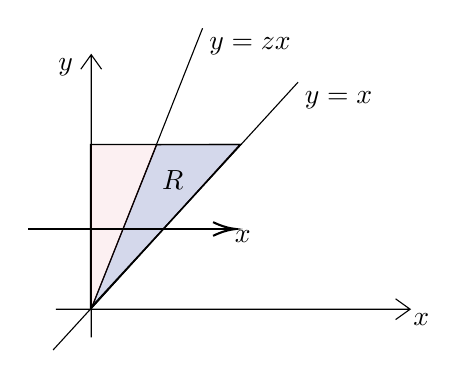
\begin{tikzpicture}[x=0.75pt,y=0.75pt,yscale=-1,xscale=1]
			\draw  (53,190.65) -- (223.73,190.65)(70.07,68) -- (70.07,204.27) (216.73,185.65) -- (223.73,190.65) -- (216.73,195.65) (65.07,75) -- (70.07,68) -- (75.07,75)  ;
			\draw    (169.73,81.27) -- (51.73,210.27) ;
			\draw    (70.07,190.65) -- (123.73,55.27) ;
			\draw    (69.73,111.27) -- (141.73,111.27) ;
			\draw  [fill={rgb, 255:red, 74; green, 144; blue, 226 }  ,fill opacity=0.23 ] (101.66,111.39) -- (141.73,111.27) -- (70.1,190.3) -- cycle ;
			\draw  [fill={rgb, 255:red, 208; green, 2; blue, 27 }  ,fill opacity=0.06 ] (142.19,111.27) -- (69.73,189.92) -- (69.73,111.27) -- cycle ;
			\draw    (39.73,152) -- (137.73,152) ;
			\draw [shift={(139.73,152)}, rotate = 180] [color={rgb, 255:red, 0; green, 0; blue, 0 }  ][line width=0.75]    (10.93,-3.29) .. controls (6.95,-1.4) and (3.31,-0.3) .. (0,0) .. controls (3.31,0.3) and (6.95,1.4) .. (10.93,3.29)   ;
			\draw (171.73,84.67) node [anchor=north west][inner sep=0.75pt]    {$y=x$};
			\draw (125.73,58.67) node [anchor=north west][inner sep=0.75pt]    {$y=zx$};
			\draw (103,122.4) node [anchor=north west][inner sep=0.75pt]    {$R$};
			\draw (138,151.4) node [anchor=north west][inner sep=0.75pt]    {$x$};
			\draw (224,191.4) node [anchor=north west][inner sep=0.75pt]    {$x$};
			\draw (53,68.4) node [anchor=north west][inner sep=0.75pt]    {$y$};
			\end{tikzpicture}
		\end{center}
		\begin{align*}\P_Z(z)=\P(Z\leq z)=\P\qty(\dfrac{Y}{X}\leq z)=\P(Y\leq zX)&=\iint_R f_{X,Y}(x,y)\ \d{x}\d{y}\\&=\int_0^1\int_{y/z}^y2\ \d{x}\d{y}\\&=\int_0^12\qty(y-\dfrac{y}{z})\ \d{y}\\&=\int_0^12\qty(1-\dfrac{1}{z})y\ \d{y}\\&=2\cdot\qty(1-\dfrac{1}{z})\cdot\dfrac{1}{2}\mqty[y^2]_0^1\\&=1-\dfrac{1}{2}\end{align*} Therefore, \[f_Z(z)=\dv{z}F_Z(z)=\dv{z}\qty(1-\dfrac{1}{z})=z^{-2},\quad z>1.\]
	\end{sol}
\end{eg}

\subsection{Combining Independent Random Variables}
\begin{rmk}
	First check for dependencies of the domain: We need rectangular relationship between $X$ and $Y$. 	
\end{rmk}
\begin{thm}{Review}
	\begin{itemize}
		\item Joint cdf: $\dsst F_{X,Y}(x,y)=\P(X\leq x, Y\leq y)=\int_{-\infty}^x\int_{-\infty}^yf_{X,Y}(s,t)\ \d{t}\d{s}$
		\item If $Y=aX+b$, then \[f_Y(y)=\dfrac{1}{\qty|a|}f_X\qty(\dfrac{y-b}{a}).\]
	\end{itemize}	
\end{thm}
\begin{thm}{Strategies for Finding New pdfs}
	\begin{itemize}
		\item Discrete pdf: compute the probability directly
		\item Continuous pdf: use the cdf $\to$ pdf method.
	\end{itemize}	
\end{thm}
\begin{eg}
	Let $X\sim\text{Binomial}(n,p)$ and $Y\sim\text{Binomial}(m,p)$. Let $X$ and $Y$ be independent. Find the pdf for $W=X+Y$.
	\begin{sol}
		\[\P_X(x)=\binom{n}{x}p^x(1-p)^{n-x};\quad \P_Y(y)=\binom{m}{y}p^y(1-p)^{m-y}\]\begin{align*}\P_W(w)=\P(W=w)&=\sum_x\underbrace{\P_X(x)\P_Y(w-x)}_{\text{Joint pdf} \P_{X,Y}(x,y),\ w=x+y}\\&=\sum_x\binom{n}{x}p^x(1-p)^{n-x}\binom{m}{w-x}p^{w-x}(1-p)^{m-(w-x)}\\&=\sum_x\binom{n}{x}\binom{m}{w-x}p^{x+w-x}(1-p)^{n-x+m-w+x}\\&=\sum_x\binom{n}{x}\binom{m}{w-x}p^{w}(1-p)^{n+m-w}\\&=p^w(1-p)^{n+m-w}\qty(\sum_x\binom{n}{x}\binom{m}{w-x})\\&=\binom{m+n}{w}p^w(1-p)^{n+m-w}\end{align*} So, $W=X+Y\sim\text{Binomial}(n+m,p)$
	\end{sol}
\end{eg}
\begin{thm}{Sum of Continuous Independent Random Variable, $W=X+Y$}
	\[f_W(w)=\int_{-\infty}^\infty f_X(x)f_Y(w-x)\ \d{x}\]	
\end{thm}
\begin{prf}
	By independence, we have \begin{align*}F_W(w)&=\P(W\leq w)\\&=\P(X+Y\leq w)\\&=\P(Y\leq w-X)\\&=\int_{-\infty}^\infty\int_{-\infty}^{w-x} f_X(x)f_Y(y)\ \d{y}\d{x}\end{align*} Then, by Fundamental Theorem of Calculus, we have \begin{align*}f_W(w)&=\dv{w}\int_{-\infty}^\infty\int_{-\infty}^{w-x}f_X(x)f_Y(y)\ \d{y}\d{x}\\&=\int_{-\infty}^\infty f_X(x)\dv{w}\int_{-\infty}^{w-x}f_Y(y)\ \d{y}\ \d{x}\\\text{convolution}&=\int_{-\infty}^\infty f_X(x)f_Y(w-x)(1)\ \d{x}\end{align*}
\end{prf}
\begin{thm}{Quotient of Continuous Independent Random Variables, $W=\dfrac{Y}{X}$}
	\[f_W(w)=\int_{-\infty}^\infty\qty|x|f_X(x)f_Y(wx)\ \d{x};\quad \dv{w}(wx)=\qty|x|\]
\end{thm}
\begin{thm}{Product of Continuous Independent Random Variables, $W=XY$}
	\[f_W(w)=\int_{-\infty}^\infty\dfrac{1}{\qty|x|}f_X(x)f_Y\qty(\dfrac{w}{x})\ \d{x},\quad x\neq0;\quad\dv{w}\qty(\dfrac{w}{x})=\dfrac{1}{\qty|x|}.\]	
\end{thm}

\subsection{Further Properties of Mean and Variance}
\begin{lem}{}
	Assume $X,Y$ are continuous random variable with joint pdf $f_{X,Y}(x,y)$ and let $g(X,Y)$ be a function of random variable $X,Y$, then \[\E(g(X,Y))=\iint_{\R^2}g(x,y)f_{X,Y}(x,y)\ \d{x}\d{y}.\]	
\end{lem}
\begin{thm}{Linearity of Expected Values}
	\[\E(X+Y)=\E(X)+\E(Y)\]	
\end{thm}
\begin{prf}
	Suppose $X$ and $Y$ are two continuous random variables, we want to examine the sum of their expected values. 
	\begin{align*}
		\E(X+Y)&=\iint_{\R^2}(x+y)f_{X,Y}(x,y)\ \d{x}\d{y}\\&=\iint_{\R^2}\qty\big[xf_{X,Y}(x,y)+yf_{X,Y}(x,y)]\ \d{x}\d{y}\\&=\iint_{\R^2}xf_{X,Y}(x,y)\ \d{y}\d{x}+\iint_{\R^2}yf_{X,Y}(x,y)\ \d{x}\d{y}\\&=\int_{-\infty}^\infty x\int_{-\infty}^\infty f_{X,Y}(x,y)\ \d{y}\ \d{x}+int_{-\infty}^\infty y\int_{-\infty}^\infty f_{X,Y}(x,y)\ \d{x}\ \d{y}\\&=\int_{-\infty}^\infty xf_X(x)\ \d{x}+\int_{-\infty}^\infty yf_Y(x)\ \d{y}=\E(X)+\E(Y).
	\end{align*}	
\end{prf}
\begin{conj}{}
	We hope the expected value of a product to be $\E(XY)=\E(X)\E(Y)$.
\end{conj}
\begin{dis}
	Take an urn with two chips numbered $1$ and $2$. Draw $2$ chips without replacement. Let $X_1=$ the value on draw $1$ and $X_2=$ the value on draw $2$. \begin{align*}\E(X_1)&=\sum_{i=1}^2i\P(X=i)=1\qty(\dfrac{1}{2})+2\qty(\dfrac{1}{2})=\dfrac{3}{2}\\\P(X_2=1)&=\P(X_2=1\mid X_1=1)\P(X_1=1)+\P(X_2=1\mid X_1=2) \P(X_1=2)=0+1\qty(\dfrac{1}{2})=\dfrac{1}{2}\\\P(X_2=2)&=\P(X_2=2\mid X_1=1)\P(X_1=1)+\P(X_2=2\mid X_1=2)\P(X_1=2)=1\qty(\dfrac{1}{2})+0=\dfrac{1}{2}\\\E(X_2)&=\sum_{i=1}^2i\P(X=i)=1\qty(\dfrac{1}{2})+2\qty(\dfrac{1}{2})=\dfrac{3}{2}\end{align*}\[\E(X_1)\E(X_2)=\qty(\dfrac{3}{2})\qty(\dfrac{3}{2})=\dfrac{9}{4};\quad \E(X_1X_2)=\E(2)=2.\] Therefore, $\E(X_1)\E(X_2)\neq \E(X_1X_2)$.
\end{dis}
\begin{thm}{Expected Value of a Product}
	If $X,Y$ are independent, then \[\E(XY)=\E(X)\E(Y).\]
\end{thm}
\begin{prf}
	Suppose $X$ and $Y$ are independent. Then, \begin{align*}\E(X,Y)&=\iint_{\R^2}xyf_{X,Y}(x,y)\ \d{x}\d{y}\\&=\iint_{\R^2}xyf_X(x)f_Y(y)\ \d{x}\d{y}&\quad Independence\\&=\qty(\int_{-\infty}^\infty xf_X(x)\ \d{x})\qty(\int_{-\infty}^\infty yf_Y(y)\ \d{y})=\E(X)\E(Y).\end{align*}	
\end{prf}
\begin{thm}{Variance of a Sum}
	\[\Var(X+Y)=\Var(X)+\Var(Y)+2\Cov(X,Y),\] where \[\Cov(X,Y)=\E(XY)-\E(X)\E(Y).\] Specially, if $X$ and $Y$ are independent, \[\Var(X+Y)=\Var(X)+\Var(Y),\] and \[\Cov(X,Y)=0.\]
\end{thm}
\begin{prf}
	Recall $\Var(X)=\E(X^2)-\E(X)^2$. Then, \begin{align*}\Var(X+Y)&=\E\qty((X+Y)^2)-\E(X+Y)^2\\&=\E\qty(X^2+Y^2+2XY)-\qty[\E(X)+\E(Y)]^2\\&=\E\qty(X^2)+\E\qty(Y^2)+2\E(XY)-\E(X)^2-\E(Y)^2-2\E(X)\E(Y)\\&=\qty[\E\qty(X^2)-\E(X)^2]+\qty[\E\qty(Y^2)-\E(Y)^2]+2\qty[\E(XY)-\E(X)\E(Y)]\\&=\Var(X)+\Var(Y)+2\qty[\E(XY)-\E(X)\E(Y)]\\&=\Var(X)+\Var(Y)+2\Cov(X,Y)\end{align*} When $X$ and $Y$ are independent, $\E(XY)=\E(X)\E(Y)$, so $\E(XY)-\E(X)\E(Y)=0$. Then, \[\Var(X+Y)=\Var(X)+\Var(Y).\]
\end{prf}
\begin{rmk}
	$\Cov(X,Y)$ does not imply $X$ and $Y$ are independent. When $\E(X)$ or $\E(Y)$ is $0$, we would have $\Cov(X,Y)=0$ as well. 	
\end{rmk}
\begin{rmk}
	Summary of Properties: 
	\begin{itemize}
		\item Always true: 
		\begin{itemize}
			\item $\E(aX+b)=a\E(X)+b$
			\item $\E(X+Y)=\E(X)+\E(Y)$
			\item $\Var(aX+b)=a^2\Var(X)$
			\item $\Var(X)=\E\qty(X^2)-\E(X)^2$
		\end{itemize}
		\item When $X$ and $Y$ are independent: 
		\begin{itemize}
			\item $\E(XY)=\E(X)\E(Y)$
			\item $\Var(X+Y)=\Var(X)+\Var(Y)$
		\end{itemize}
	\end{itemize}	
\end{rmk}

\subsection{Order Statistics}
\begin{df}{Median}
	The point where half data lies above and half below.	
\end{df}
\begin{eg}
	When all the GPAs are ordered, a number is assigned by placement in the list	
\end{eg}
\begin{df}{Max/Min}
	The largest and smallest values.	
\end{df}
\begin{df}{Percentiles}
	A score that tells you the percent of people that you scored better than.	
\end{df}
\begin{df}{$i$-th Order Statistics}
	Let $Y$ be a continuous random variable for which we have drawn a \textit{random sample} (independent and identically distributed/\textit{i.i.d.}), say we have  $y_1,y_2,\dots,y_n$. We re-order them from smallest to largest: \[y_\text{min}=y_1'\leq y_2'\leq\cdots\leq y_n'=y_\text{max}\] Define a new random variable $Y_i'$, and $Y_i'$ is called the \textit{$i$-th order statistics}. Given a random sample $Y_1,\dots,Y_n$, we define \[Y_\text{min}=\min\qty(Y_1,\dots,Y_n);\quad Y_\text{max}=\max\qty(Y_1,\dots,Y_n).\]
\end{df}
\begin{df}{Percentiles}
	For any value $p$ between $0$ and $1$, the $100p$-th percentile is the observation such that $np$ observations are less than that value, and $n(1-p)$ are greater. 
\end{df}
\begin{eg}
	Suppose a random sample $y_1=3.2,\ y_2=4,\ y_3=1.1,\ y_4=0$. Then, \[0\leq1.1\leq3.2\leq4.\] So, $Y_\text{min}=0=y_\text{min}$, $y_2'=1.1$, $y_3'=3.2$, and $y_\text{max}=4=Y_\text{max}$.
\end{eg}
\begin{eg}
	Let $Y_1,\dots,Y_n$ be a random sample from $Y\sim\text{Uniform}(0,a)$ where are do not know $a$. We can estimate $a$ by different methods. \par 
	$\boxed{\text{Method }1}$ Use the sample mean: \[\E(Y)=\mu=\dfrac{a}{2}\] So we solve for $\hat{a}\approx2\mu\approx2\overline{Y}$. Then, we can estimate $a$ with $\bar{Y}$. However, we might have $y_\text{max}\geq2\bar{Y}$ which leads to a better method.\par 
	$\boxed{\text{Method }2}$ Use observed $y_\text{max}$. We know the following inequality must hold: \[a\geq Y_\text{max}.\] To find $\E(Y_\text{max})$, we first need to find the pdf of $Y_\text{max}$. We consider the cdf$\to$pdf method: \begin{align*}F_{Y_\text{max}}(y)=\P\qty(Y_\text{max}\leq y)&=\P\qty(Y_1\leq y_1, Y_2\leq y_2, Y_3\leq y_3,\dots,Y_n\leq y_n)\\&=\P(Y_1\leq y_1)\P(Y_2\leq y_2)\cdots \P(Y_n\leq y_n)\\&=\qty(\dfrac{y}{a})^n\end{align*} So, we know \[f_{Y_\text{max}}(y)=\dv{y}F_{Y_\text{max}}(y)=\dv{y}\qty[\qty(\dfrac{y}{a})^n]=\dfrac{n}{a}\qty(\dfrac{y}{a})^{n-1}.\] So, we can find the expected value: \begin{align*}\E(Y_\text{max})=\int_0^ayf_{Y_\text{max}}(y)\ \d{y}&=\int_0^ay\dfrac{n}{a}\qty(\dfrac{y}{a})^{n-1}\ \d{y}\\&=\dfrac{n}{a^n}\int_0^ay^n\ \d{y}\\&=\dfrac{n}{a^n}\qty[\dfrac{1}{n+1}y^{n+1}]_0^a\\&=\dfrac{n}{a^n}\cdot\dfrac{1}{n+1}a^{n+1}\\&=\dfrac{n}{n+1}a\end{align*}Therefore, we can estimate $y_\text{max}=\dsst\dfrac{n}{n+1}a$. So we get $a\approx\dfrac{n+1}{n}y_\text{max}.$
\end{eg}
\begin{thm}{Order Statistics}
	\[Y_\text{max}:\ F_{Y_\text{max}}(y)=F_y(y)^n\implies f_{Y_\text{max}}(y)=nF_Y(y)^{n-1}f_Y(y).\] \[Y_\text{min}:\ F_{Y_\text{min}}(y)=1-\qty[1-F_y(y)]^n\implies f_{Y_\text{min}}(y)=n\qty[1-F_Y(y)]^{n-1}f_Y(y).\]
\end{thm}
\begin{prf}
	The formula of $Y_\text{min}$ will proven here. \begin{align*}F_{Y_\text{min}}(y)=\P(Y_\text{min}\leq y)&=1-\P(Y_\text{min}>y)\\&=1-\P(Y_1>y,Y_2>y,\dots,Y_n>y)\\&=1-\P(Y_1>y)\P(Y_2>y)\cdots \P(Y_n>y)\\&=1-[1-F_Y(y)][1-F_Y(y)]\cdots[1-F_Y(y)]\\&=1-[1-F_Y(y)]^n\end{align*} So, we would also have $f_{Y_\text{min}}(y)=n\qty[1-F_Y(y)]^{n-1}f_Y(y)$.
\end{prf}
\begin{thm}{$i$-th Order Statistics}
	\[Y_i':\ f_{Y_i'}(y)=\dfrac{n!}{(i-1)!(n-i)!}[F_Y(y)]^{i-1}[1-F_Y(y)]^{n-i}f_Y(y),\quad1\leq i\leq n.\]
\end{thm}

\subsection{Conditional Densities}
\begin{df}{Conditional Probability}
	Let $X,Y$ be discrete random variables with joint pdf $p_{X,Y}(x,y)$, then the conditional probability \[p_{Y\mid X}(y)=\P(Y=y\mid X=x)=\dfrac{p_{X,Y}(x,y)}{p_X(x)}.\]	
\end{df}
\begin{eg}
	A bag with $5$ fair coins and one $2$ headed coin. Choose a coin and flip it $n$ times. Let $X=\begin{cases}1\quad\text{if the coin is fiar}\\2\quad\text{if the two headed coin is selected}\end{cases}$	and $Y=$ the number of heads in $n$ tosses. Find $\P_Y(y)$.
	\begin{sol}
		Our plan: find $p_X(x)\implies p_{Y\mid X=1}(y),\ p_{Y\mid X=2}(y)\implies p_{X,Y}(x,y)=p_{Y\mid X}(y)p_X(x)\implies$ sum over all values of $x$ to get the $p_Y(y)$. \[p_X(x)=\begin{cases}\dfrac{5}{6}\quad X=1\\\\\dfrac{1}{6}\quad X=2\end{cases}\]\[p_{Y\mid1}(y)=\binom{n}{y}\qty(\dfrac{1}{2})^y\qty(1-\dfrac{1}{2})^{n-y}=\binom{n}{y}\qty(\dfrac{1}{2})^n\]\[p_{Y\mid2}(y)=\begin{cases}0\quad y<n\\1\quad y=n\end{cases}.\] Therefore, the joint pdf 
		\begin{center}\begin{tabular}{c|c|c|c|c}
			&$Y=0$&$Y=1$&$Y=k$&$Y=n$\\\hline
			&&&\\
			$X=1$&$\qty(\dfrac{1}{2})^{n}\qty(\dfrac{5}{6})$&$\dsst\binom{n}{1}\qty(\dfrac{1}{2})^n\qty(\dfrac{5}{6})$&$\dsst\binom{n}{k}\qty(\frac{1}{2})^n\qty(\frac{5}{6})$&$1\dsst\qty(\frac{1}{2})^n\qty(\frac{5}{6})$\\
			&&&\\
			$X=2$&$0$&$0$&$0$&$1\dsst\qty(\frac{1}{6})$\\
			&&&\\
			$p_Y(y)$&$\qty(\dfrac{1}{2})^{n}\qty(\dfrac{5}{6})$&$\dsst\binom{n}{1}\qty(\dfrac{1}{2})^n\qty(\dfrac{5}{6})$&$\dsst\binom{n}{k}\qty(\frac{1}{2})^n\qty(\frac{5}{6})$&$\dsst\qty(\frac{1}{2})^n\qty(\frac{5}{6})+\qty(\frac{1}{6})$
		\end{tabular}\end{center}
		In other words, \[p_Y(y)=\begin{cases}\dsst\qty(\dfrac{5}{6})\binom{n}{y}\qty(\dfrac{1}{2})^n\quad 0\leq y<n\\\\\qty(\dfrac{1}{2})^n\qty(\dfrac{5}{6})+\qty(\dfrac{1}{6})\quad y=n\end{cases}\]
	\end{sol}
\end{eg}
\begin{rmk}If we define the conditional density in the same way as in the discrete case, we shall have \[\dfrac{\P(X=x, Y=y)}{\P(X=x)}.\] However, $\P(X=x)=0$ when $X$ is continuous. Thus, we need an alternative definition when $X$ is continuous. \end{rmk}
\begin{df}{Conditional Probability - Continuous}
	Let $X$ and $Y$ be two continuous random variables. Then, the conditional probability \[f_{Y\mid X}(y)=\dfrac{f_{X,Y}(x,y)}{f_X(x)}.\]	
\end{df}
\begin{prf}
	We will use the cdf$\to$pdf method. Define the cdf of the conditional probability to be \begin{align*}F_{Y\mid X}(y)&=\lim_{h\to0}\P(Y\leq y\mid X\in[x,x+h])\\&=\lim_{h\to0}\dfrac{\dsst\int_x^{x+h}\int_{-\infty}^y\P_{X,Y}(s,t)\ \d{t}\d{s}}{\dsst\int_x^{x+h}f_X(s)\ \d{x}}&\dfrac{0}{0}\implies L'Hopitals'\\&=\lim_{h\to0}\dfrac{\dsst\dv{h}\int_x^{x+h}\int_{-\infty}^y\P_{X,Y}(s,t)\ \d{t}\d{s}}{\dsst\dv{h}\int_x^{x+h}f_X(s)\ \d{s}}\\&=\lim_{h\to0}\dfrac{\dsst\int_{-\infty}^y\P_{X,Y}(x+h,t)\ \d{t}}{\dsst f_X(x+h)}\\&=\dfrac{\dsst\int_{-\infty}^y\P_{X,Y}(x,t)\ \d{t}}{f_X(x)}\end{align*}	So, we know \begin{align*}f_{Y\mid X}(y)&=\dv{y}\dfrac{\dsst\int_{-\infty}^y\P_{X,Y}(x,t)\ \d{t}}{f_X(x)}\\&=\dfrac{f_{X,Y}(x,y)}{f_X(x)}.\end{align*}
\end{prf}
\begin{eg}
	A stick of unit length, and break it at a random point. Let $X=$ length of the larger piece. Then, break the larger piece, and let $Y=$ the length of the larger piece after the second break. Find $\E(Y)$.
	\begin{sol}
		Find the pdf of $X$: let $W=$ the breaking point. Assume $W\sim\text{Uniform}(0,1)$. Then, $X=\max(W,1-W)$. So we have \begin{align*}F_X(x)=\P(X\leq x)&=\P(W\leq x\text{ and }1-x\leq W)\\&=\P(W\in[1-x,x])&X\in\qty[\dfrac{1}{2},1]\\&=\int_{1-x}^x1\ \d{w}=2x-1\\f_X(x)=\dv{x}F_X(x)&=\dv{x}[2x-1]=2.\end{align*} Find the joint pdf: repeat the same process for $Y\mid X\sim\text{Uniform}\qty(\dfrac{X}{2},X)$. We have \begin{align*}f_{Y\mid X}(y)&=\dfrac{1}{x-\frac{x}{2}}=\dfrac{2}{x}&y\in\qty[\dfrac{x}{2},x]\\f_{X,Y}(x,y)&=f_{Y\mid X}(y)f_X(x)\\&=\dfrac{2}{x}\cdot2=\dfrac{4}{x}.&x\in\qty[\dfrac{1}{2},1],\ y\in\qty[\dfrac{x}{2},x]\end{align*} Now, we can find the expected value: \begin{align*}\E(Y)&=\int_{1/2}^1\int_{x/2}^xyf_{X,Y}(x,y)\ \d{y}\d{x}\\&=\int_{1/2}^1\int_{x/2}^xy\dfrac{4}{x}\ \d{y}\d{x}\\&=\int_{1/2}^1\dfrac{4}{x}\qty[\dfrac{1}{2}y^2]_{x/2}^x\ \d{x}\\&=\int_{1/2}^1\dfrac{2}{x}\qty(x^2-\dfrac{x^2}{4})\ \d{x}\\&=\int_{1/2}^1\dfrac{3}{2}x\ \d{x}\\&=\dfrac{3}{2}\qty[\dfrac{1}{2}x^2]_{1/2}^1\\&=\dfrac{3}{4}\qty(1-\dfrac{1}{4})=\dfrac{9}{16}.\end{align*}
	\end{sol}
\end{eg}

\subsection{Moment Generating Functions (mgf)}
\begin{df}{Moment}
	The moments of the distribution of $X$ are \[\E\qty(X^k)\quad\text{for }k=1,2,\dots\] if they exists. The mean $\mu$ is the first moment. 
\end{df}
\begin{df}{Moment Generating Functions/mgf}
	\[\M_X(t)=\E\qty(e^{tX})=\begin{cases}\dsst\sum_ke^{tk}p_X(k)\quad\text{if }X\text{ is discrete}\\\\\dsst\int_{-\infty}^\infty e^{tx}f_X(x)\ \d{x}\quad\text{if }X\text{ is continuous}\end{cases}\]	
\end{df}
\begin{rmk}
	Why we would use $\E\qty(e^{tX})$?\par Recall the Macluarin Series expansion for \[e^{tX}=\sum_{n=0}^\infty\dfrac{(tX)^n}{n!}=1+tX+\dfrac{(tX)^2}{2!}+\dfrac{(tX)^3}{3!}+\cdots\] Then, we have \begin{align*}\M_X(t)=\E\qty(e^{tX})=\E\qty(\sum_{n=0}^\infty\dfrac{(tX)^n}{n!})&=\sum_{n=0}^\infty\E\qty(\dfrac{t^nx^n}{n!})\\&=\sum_{n=0}^\infty\dfrac{t^n}{n!}\E\qty(X^n)\\&=1+t\E(X)+\dfrac{t^2}{2!}\E\qty(X^2)+\dfrac{t^3}{3!}\E\qty(X^3)+\cdots\\&=1+tm_1+\dfrac{t^2}{2!}m_2+\dfrac{t^3}{3!}m_3+\cdots\\&=1+m_1t+\dfrac{m_2}{2!}t^2+\dfrac{m_3}{3!}t^3+\cdots\end{align*}
\end{rmk}
\begin{eg}
	Recover $m_1$ from the moment generating function.\par $\boxed{\text{Step }1}$ Differentiate $\M_X(t)$ with respect to $t$. \[\M_X(t)=1+m_1t+\dfrac{m_2}{2!}t^2+\dfrac{m_3}{3!}t^3+\cdots\]\[\M_X^{(1)}(t)=0+m_1+\dfrac{2m_2}{2!}t+\dfrac{3m_3}{3!}t^2+\cdots=m_1+m_2t+\dfrac{m_3}{2!}t^2+\cdots\]\par $\boxed{\text{Step }2}$ Evaluate $t=0$: Higher order terms drop out when $t=0$.\[\M_X^{(1)}(0)=m_1\]
	\end{eg}
\begin{thm}{}
	\[\M_Y^{(n)}(0)=\E\qty(Y^n)\quad\text{as long as }\E\qty(Y^n)<\infty.\]
\end{thm}
\begin{eg}
	Recover $m_2$: \[\M_X^{(2)}(t)=0+m_2+\dfrac{2m_3}{2!}t+\cdots=m_2+m_3t+\cdots\implies\M_X^{(2)}(0)=m_2.\]
\end{eg}
\begin{thm}{}
	If $Y_1$ and $Y_2$ have $\M_{Y_1}(t)=\M_{Y_2}(t)$ for an open interval of $t$ about $0$, then the pdf's are identical. i.e., $f_{Y_1}(y)=f_{Y_2(y)}$.	
\end{thm}
\begin{thm}{Properties of mgf}
	\begin{itemize}
		\item If $Y=aX+b$, then \[\M_Y(t)=e^{bt}\M_X(at)\]
		\item If $W=X+Y$ and $X,Y$ are independent, then \[\M_W(t)=\M_X(t)\cdot\M_Y(t).\] This is much easier than computing $f_W(w)=f_X\cdot f_Y$.
	\end{itemize}
\end{thm}
\begin{eg}
	Let $Y\sim N(0,1)$ (Normal with $\mu=0$ and $\sigma^2=1$). Find the mgf for $W\sim N(\mu,\sigma^2)$.
	\begin{sol}
		We have that $f_Y(y)=\dfrac{1}{\sqrt{2\pi}}e^{-y^2/2},\quad y\in(-\infty,\infty).$\begin{align*}\M_Y(t)=\E\qty(e^{tY})=\int_{-\infty}^\infty e^{ty}\dfrac{1}{\sqrt{2\pi}}e^{-y^2/2}\ \d{y}&=\dfrac{1}{\sqrt{2\pi}}\int_{-\infty}^\infty e^{ty-y^2/2}\ \d{y}\\&=\dfrac{1}{\sqrt{2\pi}}\int_{-\infty}^\infty e^{-\frac{1}{2}(y-t)^2+t^2/2}\ \d{y}\\&=\dfrac{1}{\sqrt{2\pi}}\int_{-\infty}^\infty e^{-\frac{1}{2}(y-t)^2}e^{t^2/2}\ \d{y}\\&=e^{t^2/2}\underbrace{\dfrac{1}{\sqrt{2\pi}}\int_{-\infty}^\infty e^{-\frac{1}{2}(y-t)^2\ \d{y}}}_{\text{pdf of }Y\text{ shift by }t\text{ unit}=1}\\&=e^{t^2/2}\end{align*} $W=\sigma Y+\mu$, then by the property of mgf, we have \[\M_W(t)=e^{\mu t}\M_Y(\sigma t)=e^{\mu t}e^{(\sigma t)^2/2}=e^{\frac{!}{2}\sigma^2t^2+\mu t}.\]

	\end{sol}
\end{eg}

\newpage
\section{Special Distributions}
\subsection{Poisson Distribution}
\begin{eg}
	A publisher estimates that their books have an average $1$ typo every $4$ pages. Let $X=$ number of typos in a $20$ page chapter. Assume: (1) the typos are equally likely to occur anywhere, (2) different typos are independent, and (3) average rate of the typos is $\dfrac{1}{4}$ per page. 
	\begin{enumerate}
		\item[a.] Let $X_j=$ \# of typos on page $j$. 
		\begin{sol}
			Expect $\dfrac{1}{4}$ per page $\implies p_X(k)=\begin{cases}1/4\quad k=1\\3/4\quad k=0\end{cases}$.\par  Then, $X_j\sim\text{Binomial}\qty(n=20,p=\dfrac{1}{4})$. So, \[\P(X=k)=\binom{20}{k}\qty(\dfrac{1}{4})^k\qty(\dfrac{3}{4})^{20-k}\] Therefore, \[\P(X=5)=\binom{20}{5}\qty(\dfrac{1}{4})^5\qty(\dfrac{3}{4})^{15}\approx20.2\%\]
			Problem: maximum \# of typo is $20$, but we can have more typos per page!	
		\end{sol}
		\item[b.] Subdivide each page into $40$ lines. $\implies n=800$ total lines and $p=\dfrac{1/4}{40}=\dfrac{1}{160}$. 
		\begin{sol}
			Let $X_j=$ \# of typos on line $j$. Then, $X_j\sim\text{Binomial}\qty(n=800,p=\dfrac{!}{160})$. So, \[p_{X_j}(k)=\binom{800}{k}\qty(\dfrac{1}{160})^k\qty(\dfrac{159}{160})^{800-k},\quad k=0,\dots,800\]\[\P\qty(X_j=5)=17.6\%\]	
		\end{sol}
		\item[c.] Subdivide each line into quarter lines. That is, $n=3200$ quarter lines and $p=\dfrac{1}{640}$.
		\begin{sol}
			$X_j=$ a typo on quarter line $j$. So, $X_j\sim\text{Binomial}\qty(3200,\dfrac{1}{640})$. \[p_{X_j}(k)=\binom{3200}{k}\qty(\dfrac{1}{640})^k\qty(\dfrac{639}{640})^{3200-k}.\]	
		\end{sol}
		\item[d.] Does this approach a limit? Let $\lambda=$ total \# expected, $n=$ \# of subdivisions, $p=\dfrac{\lambda}{n}$ probability within one division. Then, $\dsst p_X(k)=\binom{n}{k}\qty(\dfrac{\lambda}{n})^k\qty(1-\dfrac{\lambda}{n})^{n-k}$. Fix $k$ and $\lambda$. Find $\dsst\lim_{n\to\infty}p_X(k)$.
		\begin{sol}
			\begin{align*}
				\lim_{n\to\infty}p_X(k)&=\lim_{n\to\infty}\binom{n}{k}\qty(\dfrac{\lambda}{n})^k\qty(1-\dfrac{\lambda}{n})^{n-k}\\
				&=\lim_{n\to\infty}\dfrac{n!}{(n-k)!k!}\cdot\dfrac{\lambda^k}{n^k}\qty(1-\dfrac{\lambda}{n})^n\qty(1-\dfrac{\lambda}{n})^{-k}\\
				&=\dfrac{\lambda^k}{k!}\lim_{n\to\infty}\dfrac{n!}{(n-k)!}\cdot\dfrac{1}{n^k\qty(1-\frac{\lambda}{n})^k}\cdot\qty(1-\dfrac{\lambda}{n})^n\\
				&=\dfrac{\lambda^k}{k!}\lim_{n\to\infty}\dfrac{n(n-1)\cdots(n-k+1)(n-k)!}{(n-k)!(n-\lambda)^k}\cdot\qty(1-\dfrac{\lambda}{n})^n\\
				&=\dfrac{\lambda^k}{k!}\lim_{n\to\infty}\underbrace{\dfrac{n(n-1)\cdots(n-k+1)}{(n-\lambda)^k}}_{\sim\lim_{n\to\infty}\frac{n^k}{n^k}=1}\underbrace{\qty(1-\dfrac{\lambda}{n})^n}_{=\lim_{n\to\infty}e^{-\lambda}}\\
				&=\dfrac{\lambda^k}{k!}e^{-\lambda}
			\end{align*}
		\end{sol}
	\end{enumerate}	
\end{eg}
\begin{df}{Poisson Distribution}
	For $X\in\N$ and $\lambda>0$, the pdf of \textit{poisson distribution} is given by \[p_X(k)=P(X=k)=e^{-\lambda}\dfrac{\lambda^k}{k!},\quad\text{for }k=0,1,2,\dots\]
\end{df}
\begin{df}{Poisson Model}
	Assume the events occur with the following assumptions: 
	\begin{itemize}
		\item Can subdivide into intervals small enough that $\P(2\text{ events in one interval})=0$.
		\item Occurrences in different intervals are independent.
		\item Probability of event is constant.
	\end{itemize}
	Then, set $\lambda=$ expected \# of occurrence per unit and $X=$ actual \# of occurrence per unit. Then, we have the \textit{poisson model}: \[\P(X=k)=e^{-\lambda}\dfrac{\lambda^k}{k!}\]
\end{df}
\begin{eg}
	Application of Poisson Distribution
	\begin{enumerate}
		\item Radioactive decay (or other discrete reactions).
		\item Errors/flaws/accidents injuries
		\item Outbreaks of non-contagious disease.
	\end{enumerate}
\end{eg}
\begin{eg}
	Wait time Between Poisson Distribution\par Suppose we use a geiger counter to measure the radiation coming off a radioactive sample. The number of ticks in $1$ second of the counter has a poisson distribution, where $\lambda$ is the expected number of ticks, i.e., $\lambda=$ average number of ticks per second. Let $Y=$ the time interval between two consecutive ticks. What is the distribution of $Y$? 
	\begin{sol}
		The cdf of $Y$: $F_Y(y)=\P(Y\leq y).$\par Let $t=0$ be the time of the first click. Then, $Y\leq y$ can be interpreted as at least $1$ click in $[0,y]$. So, we have \[F_Y(y)=1-\P(\text{No clicks in }[0,y]).\] The expected number of clicks is $\lambda y\implies\P(\text{none})=e^{-\lambda y}$. Thus, \[F_Y(y)=1-e^{-\lambda y}.\] So, the pdf of $Y$ is given by \[f_Y(y)=\dv{y}F_Y(y)=\lambda e^{-\lambda y},\quad y\geq0\]
	\end{sol}
\end{eg}
\begin{thm}{Wait Time Between Poisson Distribution}
	Suppose a series of events satisfying the poisson distribution	model are occurring at the rate of $\lambda$ units per time. Let random variable $Y$ denote the interval between consecutive events. Then, $Y$ has the exponential distribution: $Y\sim\text{Exponential}(\lambda)$, and \[f_Y(y)=\lambda e^{-\lambda y},\quad y>0.\]
\end{thm}

\subsection{Normal Distribution}
\begin{df}{The Standard Normal}
	A continuous random variable $Z\sim N(0,1)=\text{Normal}\qty(\mu=0,\sigma^2=1)$	is defined to be the standard normal distribution with pdf \[f_Z(z)=\dfrac{1}{\sqrt{2\pi}}e^{-z^2/2},\quad z\in(-\infty, \infty)\] and the moment generating function \[\M_Z(t)=e^{t^2/2},\quad t\in\R\] The standard normal distribution is also known as the Gaussian distribution or the bell curve. 
\end{df}
\begin{df}{The General Normal Distribution}
	We define the general normal distribution $X\sim N(\mu,\sigma^2)$ by using the transformation $X=\sigma Z+\mu$. Any normal distribution is a linear transformation of the standard normal, and the pdf is given by \[f_X(x)=\dfrac{1}{\sqrt{a\pi}\sigma}e^{-\frac{1}{2\sigma^2}(x-\mu)^2},\quad x\in\R\]
\end{df}
\begin{prf}
	Note that the cdf of $X=\sigma Z+\mu$ is given by \begin{align*}F_X(x)=\P(X\leq x)&=\P(\sigma Z+\mu\leq x)\\&=\P\qty(Z\leq\dfrac{x-\mu}{\sigma})=F_Z\qty(\dfrac{x-\mu}{\sigma})\end{align*} So, the pdf of $X$ is \begin{align*}f_X(x)=\dv{x}F_X(x)&=\dv{x}F_Z\qty(\dfrac{x-\mu}{\sigma})\\&=f_Z\qty(\dfrac{x-\mu}{\sigma})\cdot\dv{x}\qty(\dfrac{x}{\sigma}-\dfrac{\mu}{\sigma})\\&=\dfrac{1}{\sqrt{2\pi}}e^{-\qty(\frac{x-\mu}{\sigma})^2\cdot\frac{1}{2}}\qty(\dfrac{1}{\sigma})\\&=\dfrac{1}{\sqrt{2\pi}\sigma}e^{-\frac{1}{2\sigma^2}(x-\mu)^2},\quad x\in\R\end{align*}
\end{prf}
\begin{rmk} Using the MGF that if $\mathrm{Normal}+\mathrm{Normal}=\mathrm{Normal}$.\end{rmk}
\begin{eg}{}
	Applications of Normal Distribution
	\begin{itemize}
		\item Sample means
		\item Population features
		\item Lab instrument measures
	\end{itemize}	
\end{eg}
\begin{eg}
	Why $\dfrac{1}{\sqrt{2\pi}}$?
	\begin{sol}
		We want to compute $\dsst\int_{-\infty}^\infty e^{-x^2/2}\ \d{x}$. Instead of finding it directly, we can find \begin{align*}\qty(\int_{-\infty}^\infty e^{-x^2/2}\ \d{x})^2&=\int_{-\infty}^\infty e^{-x^2/2}\ \d{x}\int_{-\infty}^\infty e^{-y^2/2}\ \d{y}\\&=\int_{-\infty}^\infty\int_{-\infty}^\infty e^{-(x^2+y^2)/2}\ \d{x}\d{y}.\end{align*} Use the polar coordinate: $x=r\cos\theta$ and $y=r\sin\theta$. So, we have $\d{x}\d{y}=r\d{r}\d{\theta}$. So, \begin{align*}\qty(\int_{-\infty}^\infty e^{-x^2/2}\ \d{x})^2&=\int_0^{2\pi}\int_0^{\infty}e^{-\qty(r^2\cos^2\theta+r^2\sin^2\theta)/2}r\ \d{r}\d{\theta}\\&=\int_0^{2\pi}\int_0^{\infty}e^{-\frac{1}{2}r^2\qty(\cos^2\theta+\sin^2\theta)}r\ \d{r}\d{\theta}\\&=\int_0^{2\pi}\int_0^{\infty}re^{-\frac{1}{2}r^2}\ \d{r}\d{\theta}&u=\frac{1}{2}r^2,\quad \d{u}=r\d{r}\\&=\int_0^{\pi}\int_0^\infty e^{-u}\ \d{u}\d{\theta}\\&=\int_0^{2\pi}\lim_{t\to\infty}\qty[-e^{-u}]_0^t\ \d{\theta}\\&=\int_0^{2\pi}\lim_{t\to\infty}\qty(-e^{-t}+e^{-0})\ \d{\theta}\\&=\int_0^{2\pi}\ \d{\theta}\\&=\qty\Big[\theta]_0^{2\pi}=2\pi\end{align*} Therefore, $\dsst\int_{-\infty}^\infty e^{-x^2/2}\ \d{x}=\sqrt{2\pi}$. Thus, to ensure the area under the pdf goes to $1$, we need the factor $\dfrac{1}{\sqrt{2\pi}}$.
	\end{sol}
\end{eg}
\begin{thm}{Central Limit Theorem}
	Let $Y_1,\dots,Y_n$ be a random sample with $\mu=\E\qty(Y_i)$ and $\sigma^2=\Var\qty(Y_i)$, both finite. Then, if \[Z_n=\dfrac{1}{\sqrt{n}\sigma}\qty(Y_1+\cdots+Y_n-n\mu),\]	 we have \[\P(a\leq Z_n\leq b)=\int_a^b\dfrac{1}{\sqrt{2\pi}}e^{-z^2/2}\ \d{z}\quad \text{as }n\to\infty\] That is, $Z_n$ approaches the standard normal as $n\to\infty$.
\end{thm}
\begin{prf}
	Tools used in this proof: MGF determines the distribution. If $\M_{Z_n}(t)\to\M_Z(t)$, then $\P(a\leq Z_n\leq b)\to\P(a\leq Z\leq b)$. \par 
	Given $Y_1,Y_2,\dots,Y_n$ a random sample as above. Let's define \[W_i=\dfrac{1}{\sigma}\qty(Y_i-\mu).\] Then, \[\E\qty(W_i)=0\qquad\text{and}\qquad\Var\qty(W_i)=1\] Assume the MGF of $W_i$ is well-defined. Without loss of generality, consider the MGF of $W_i$: \begin{align*}\M_{W_i}(t)&=e^{\phi(t)}\\\M_{W_i}(0)&=e^{\phi(0)}=1&by\ well\ defined\\\M_{W_i}'(t)&=e^{\phi(t)}\phi'(t)\\\M'_{W_i}(t)&=e^{\phi(0)}\phi'(0)=\E\qty(W_i)=0\\&\quad 1\cdot\phi'(0)=0\implies\phi'(0)=0\\\M_{W_i}''(t&)=\dv{t}\qty[e^{\phi(t)}\phi'(t)]\\&=e^{\phi(t)}\phi'(t)\phi'(t)+e^{\phi(t)}\phi''(t)\\&=e^{\phi(t)}\qty[\qty(\phi'(t))^2+\phi''(t)]\\\M_{W_i}''(0)&=^{\phi(0)}\qty[\qty(\phi'(0))^2+\phi''(0)]\\&=1\cdot\qty(0+\phi''(0))=\phi''(0)\end{align*} So, \[\Var\qty(W_i)=\E\qty(W_i^2)-\E\qty(W_i)^2=\E\qty(W_i^2)-0=\E\qty(W_i^2)=\M_{W_i}''(0)=1\] \[\implies\phi''(0)=1.\]\par 
	Now, define \[Z_n=\dfrac{1}{\sqrt{n}}\qty(W_1+W_2+\cdots+W_n).\] By the MGF property that if $X$ and $Y$ are independent, then \[\M_{aX}(t)=\M_X(at)\quad\text{and}\quad\M_{X+Y}(t)=\M_X(t)\M_Y(t)\] We have \[\M_{Z_n}(t)=\prod_{i=1}^n\M_{W_i}\qty(t/\sqrt{n})=\prod_{i=1}^ne^{\phi\qty(t/\sqrt{n})}=\qty(e^{\phi\qty(t/\sqrt{n})})^n=e^{n\phi\qty(t/\sqrt{n})}\] With $x=\dfrac{1}{\sqrt{n}}$, consider \begin{align*}\lim_{n\to\infty}n\phi\qty(t/\sqrt{n})=\lim_{n\to\infty}\dfrac{\phi(xt)}{x^2}\quad\qty(=\dfrac{0}{0})=\lim_{n\to\infty}\dfrac{\phi'(xt)t}{2x}\quad\qty(=\dfrac{0}{0})=\lim_{n\to\infty}\dfrac{\phi''(xt)t^2}{2}=\dfrac{t^2}{2}.\end{align*} That is $\dsst\lim_{n\to\infty}\M_{Z_n}(t)=e^{t^2/2}=\M_Z(t)$, the standard normal MGF. 
\end{prf}
\begin{eg} 
	Binomial Distribution and the Central Limit Theorem\par 
	Consider $X\sim\text{Binomial}(n,p)$. Note that \[X=X_1+X_2+\cdots+X_n,\quad\text{where }X_i\sim\text{Bernoulli}(p).\] So, \[Z=\dfrac{X-np}{\sqrt{np(1-p)}}\sim N(0,1)\]
\end{eg}
\begin{eg}
	Poisson Distribution and the Central Limit Theorem\par 
	Consider $X\sim\text{Poisson}(\lambda)$. Suppose \[X=X_1+X_2+\cdots+X_n,\quad\text{where }X_i\sim\text{Poisson}\qty(\dfrac{\lambda}{n})\] Then, \[Z=\dfrac{X-\lambda}{\sqrt{\lambda}}\sim N(0,1).\]
\end{eg}
\begin{rmk}
	What we are doing here is to approximate discrete distributions (e.g. binomial/poisson) with a continuous distribution (normal). There will be some errors. So we need \emph{continuity correction}, adding or subtracting $\dfrac{1}{2}$ to account for approximations of a discrete distribution with a continuous distribution.	
\end{rmk}
\begin{eg}
	Binomial Distribution Continuity Correction\par 
	\[Z=\dfrac{X-np}{\sqrt{np(1-p)}}\sim N(0,1)\] \[\P(a\leq Z\leq b)\approx\P\qty(\dfrac{a-0.5-np}{\sqrt{np(1-p)}}\leq Z\leq\dfrac{b+0.5-np}{\sqrt{np(1-p)}}).\]
\end{eg}

\subsection{CDF Tricks}
\begin{rmk}[Key idea]
	The key idea here is that we can use a cdf to generate a random sample.	
\end{rmk}
\begin{eg}
	We can let $U\sim\text{Uniform}(0,1)$ and compute $X=F_X^{-1}(U)$. Here we note that \[F_U(u)=P(U\leq u)=u.\]	 Then, we have the following: \begin{align*}F_X(x)=P(X\leq x)=P\qty(F_X^{-1}(u)\leq x)&=P\qty(F_X\qty(F_X^{-1}(U))\leq F_X(x))\\&=P(U\leq F_X(x))\\&=F_U(F_X(x))\\&=F_X(x)\end{align*}
\end{eg}
\begin{thm}{}
	We can use a uniform random sample $\text{Uniform}(0,1)$ to simulate a random variable with cdf $F_X(x)$ by setting $X=F_X^{-1}(U)$.
\end{thm}
\begin{eg}
	Simulate from the density $\dsst f_Y(y)=\dfrac{2\theta^2}{y^3},\quad y\geq\theta$.
	\begin{sol}
		$\boxed{\text{Step }1}$ Find the cdf. \begin{align*}F_Y(y)=P(Y\leq y)=\int_{\theta}^yf_Y(t)\ \d{t}=\int_\theta^y\dfrac{2\theta^2}{t^3}\ \d{t}&=2\theta^2\int_\theta^yt^{-3}\ \d{t}\\&=2\theta^2\qty[-\dfrac{1}{2}t^{-2}]_\theta^y\\&=\theta^2\qty(-y^{-2}+\theta^{-2})\\&=1-\dfrac{\theta^2}{y^2},\quad y\geq\theta\end{align*}\par 
		$\boxed{\text{Step }2}$ Find the inverse of the cdf: \begin{align*}u=F_Y(y)\implies u&=1-\dfrac{\theta^2}{y^2}\\\dfrac{\theta^2}{y^2}&=1-u\\\dfrac{1}{y^2}&=\dfrac{1-u}{\theta^2}\\y^2&=\dfrac{\theta^2}{1-u}\\y&=\sqrt{\dfrac{\theta^2}{1-u}}=\dfrac{\theta}{\sqrt{1-u}}\end{align*} Now, evaluating the above with a value of $u$ will give us a value of $y$.\par 
		$\boxed{\text{Step }3}$ Turn it into \texttt{R} code. 
	\end{sol}
\end{eg}



\end{document}